% This is the Reed College LaTeX thesis template. Most of the work
% for the document class was done by Sam Noble (SN), as well as this
% template. Later comments etc. by Ben Salzberg (BTS). Additional
% restructuring and APA support by Jess Youngberg (JY).
% Your comments and suggestions are more than welcome; please email
% them to cus@reed.edu
%
% See https://www.reed.edu/cis/help/LaTeX/index.html for help. There are a
% great bunch of help pages there, with notes on
% getting started, bibtex, etc. Go there and read it if you're not
% already familiar with LaTeX.
%
% Any line that starts with a percent symbol is a comment.
% They won't show up in the document, and are useful for notes
% to yourself and explaining commands.
% Commenting also removes a line from the document;
% very handy for troubleshooting problems. -BTS

% As far as I know, this follows the requirements laid out in
% the 2002-2003 Senior Handbook. Ask a librarian to check the
% document before binding. -SN

%%
%% Preamble
%%
% \documentclass{<something>} must begin each LaTeX document
\documentclass[12pt,oneside]{reedthesis}
% Packages are extensions to the basic LaTeX functions. Whatever you
% want to typeset, there is probably a package out there for it.
% Chemistry (chemtex), screenplays, you name it.
% Check out CTAN to see: https://www.ctan.org/
%%
\usepackage{graphicx,latexsym}
\usepackage{amsmath}
\usepackage{amssymb,amsthm}
\usepackage{longtable,booktabs,setspace}
\usepackage{chemarr} %% Useful for one reaction arrow, useless if you're not a chem major
\usepackage[hyphens]{url}
% Added by CII
\usepackage[hidelinks]{hyperref}
\usepackage{lmodern}
\usepackage{float}
\floatplacement{figure}{H}
% Thanks, @Xyv
\usepackage{calc}
% End of CII addition
\usepackage{rotating}

% Next line commented out by CII
%%% \usepackage{natbib}
% Comment out the natbib line above and uncomment the following two lines to use the new
% biblatex-chicago style, for Chicago A. Also make some changes at the end where the
% bibliography is included.
%\usepackage{biblatex-chicago}
%\bibliography{thesis}
% \ifxetex
%   \usepackage{polyglossia}
%   \setmainlanguage{spanish}
%   % Tabla en lugar de cuadro
%   \gappto\captionsspanish{\renewcommand{\tablename}{Tabla}
%           \renewcommand{\listtablename}{Índice de tablas}}
% \else
%   \usepackage[spanish,es-tabla]{babel}
% \fi

% Added by CII (Thanks, Hadley!)
% Use ref for internal links
\renewcommand{\hyperref}[2][???]{\autoref{#1}}
\def\chapterautorefname{chapter}
\def\sectionautorefname{section}
\def\subsectionautorefname{subsection}
% End of CII addition

% Added by CII
\usepackage{caption}
\captionsetup{width=5in}
% End of CII addition

% \usepackage{times} % other fonts are available like times, bookman, charter, palatino

% Syntax highlighting #22

% To pass between YAML and LaTeX the dollar signs are added by CII
\title{Ondas de Rossby planetarias en la circulación atmosférica del hemisferio sur y su influencia en Sudamérica}
\author{Lic. Elio Campitelli}
% The month and year that you submit your FINAL draft TO THE LIBRARY (May or December)
\date{BUENOS AIRES, 2023}
\division{Facultad de Ciencias Exactas y Naturales}
\advisor{Carolina Vera}
\institution{Universidad de Buenos Aires}
\degree{Tesis presentada para optar al título de Doctore de la Universidad de Buenos Aires en el Área de Ciencias de la Atmósfera y los Océanos}
%If you have two advisors for some reason, you can use the following
% Uncommented out by CII
\altadvisor{Leandro Diaz}
\consejere{Claudio Menendez}
\place{Centro de Investigaciones del Mar y la Atmósfera. CONICET-UBA}
% End of CII addition

%%% Remember to use the correct department!
\department{Departamento de Ciencias de la Atmósfera y los Océanos}
% if you're writing a thesis in an interdisciplinary major,
% uncomment the line below and change the text as appropriate.
% check the Senior Handbook if unsure.
%\thedivisionof{The Established Interdisciplinary Committee for}
% if you want the approval page to say "Approved for the Committee",
% uncomment the next line
%\approvedforthe{Committee}

% Added by CII
%%% Copied from knitr
%% maxwidth is the original width if it's less than linewidth
%% otherwise use linewidth (to make sure the graphics do not exceed the margin)
\makeatletter
\def\maxwidth{ %
  \ifdim\Gin@nat@width>\linewidth
    \linewidth
  \else
    \Gin@nat@width
  \fi
}
\makeatother

\makeatletter
\renewcommand{\@chapapp}{Capítulo}
\makeatother

% From {rticles}
\newlength{\csllabelwidth}
\setlength{\csllabelwidth}{3em}
\newlength{\cslhangindent}
\setlength{\cslhangindent}{1.5em}
% for Pandoc 2.8 to 2.10.1
\newenvironment{cslreferences}%
  {}%
  {\par}
% For Pandoc 2.11+
% As noted by @mirh [2] is needed instead of [3] for 2.12
\newenvironment{CSLReferences}[2] % #1 hanging-ident, #2 entry spacing
 {% don't indent paragraphs
  \setlength{\parindent}{0pt}
  % turn on hanging indent if param 1 is 1
  \ifodd #1 \everypar{\setlength{\hangindent}{\cslhangindent}}\ignorespaces\fi
  % set entry spacing
  \ifnum #2 > 0
  \setlength{\parskip}{#2\baselineskip}
  \fi
 }%
 {}
\usepackage{calc} % for calculating minipage widths
\newcommand{\CSLBlock}[1]{#1\hfill\break}
\newcommand{\CSLLeftMargin}[1]{\parbox[t]{\csllabelwidth}{#1}}
\newcommand{\CSLRightInline}[1]{\parbox[t]{\linewidth - \csllabelwidth}{#1}}
\newcommand{\CSLIndent}[1]{\hspace{\cslhangindent}#1}

\renewcommand{\contentsname}{Índice}
% End of CII addition

\setlength{\parskip}{0pt}

% Added by CII

\providecommand{\tightlist}{%
  \setlength{\itemsep}{0pt}\setlength{\parskip}{0pt}}

\Acknowledgements{
I want to thank a few people.
}

\Dedication{
You can have a dedication here if you wish.
}

\Preface{

}

\Abstract{
asbal albal

fdsg dfg sdfg
}


\Resumen{
Este trabajo tiene como objetivo avanzar en la caracterización y entendimiento de la circulación zonalmente asimétrica del Hemisferio Sur en escalas estacionales y más largas.
Para esto se analizaron datos de reanálisis de ERA5 y corridas históricas de CMIP6.
Se computaron las Funciones Empíricas Ortogonales Complejas (cEOF, por sus siglas en inglés) de las anomalías zonales de altura geopotencial en 200 hPa y 50 hPa.
Éstas son similares a las EOF tradicionales pero permiten caracterizar patrones de variabilidad que tienen fase además de amplitud.

El cEOF1 representa la variabilidad de la onda zonal 1 en la estratosfera y está estrechamente con las anomalías en el ozono.
El cEOF2, por su parte, representa un patrón de onda 3 con magnitud máxima en el sector del Pacífico, que resulta ser una descripción alternativa de los modos PSA.
El análisis de este modo indica que se trata de un modo de variabilidad interna de la atmósfera subtropical que toma una fase preferencial en respuesta al forzante tropical.
Sólo el cEOF2 está asociado a impactos en la superficie.

Para estudiar la relación entre estos modos de variabilidad en la circulación asimétrica y el Modo Anular del Sur (SAM), que representa principalmente variabilidad simétrica, separamos la variabilidad del SAM en su parte zonalmente simétrica (S-SAM) y asimétrica (A-SAM).
En base a la separación del SAM en S-SAM y A-SAM, observamos que la fase de 90º del cEOF2 tiene una correlación extremadamente alta con el A-SAM, sugiriendo que se trata de dos metodologías que observan el mismo fenómeno o que la parte asimétrica del SAM sea en realidad una contaminación estadística del modo PSA en un SAM más zonalmente simétrico.

Finalmente, analizamos estos modos de variabilidad en las corridas históricas del CMIP6.
Encontramos que la representación de los modos es muy variable entre modelos e incluso entre los miembros de un mismo modelo, sin embargo, la media multimodelo representa los modos muy bien.
Sin embargo, la mayoría de los modelos exageran la relación entre los modos y la temperatura de la superficie del mar
}

	\usepackage{setspace}\onehalfspacing
\usepackage[spanish,es-tabla]{babel}
	\usepackage{booktabs}
\usepackage{longtable}
\usepackage{array}
\usepackage{multirow}
\usepackage{wrapfig}
\usepackage{float}
\usepackage{colortbl}
\usepackage{pdflscape}
\usepackage{tabu}
\usepackage{threeparttable}
\usepackage{threeparttablex}
\usepackage[normalem]{ulem}
\usepackage{makecell}
\usepackage{xcolor}
% End of CII addition
%%
%% End Preamble
%%
%
\begin{document}

% Everything below added by CII
  \maketitle

\frontmatter % this stuff will be roman-numbered
\pagestyle{empty} % this removes page numbers from the frontmatter

  \begin{resumen}
    Este trabajo tiene como objetivo avanzar en la caracterización y entendimiento de la circulación zonalmente asimétrica del Hemisferio Sur en escalas estacionales y más largas.
    Para esto se analizaron datos de reanálisis de ERA5 y corridas históricas de CMIP6.
    Se computaron las Funciones Empíricas Ortogonales Complejas (cEOF, por sus siglas en inglés) de las anomalías zonales de altura geopotencial en 200 hPa y 50 hPa.
    Éstas son similares a las EOF tradicionales pero permiten caracterizar patrones de variabilidad que tienen fase además de amplitud.

    El cEOF1 representa la variabilidad de la onda zonal 1 en la estratosfera y está estrechamente con las anomalías en el ozono.
    El cEOF2, por su parte, representa un patrón de onda 3 con magnitud máxima en el sector del Pacífico, que resulta ser una descripción alternativa de los modos PSA.
    El análisis de este modo indica que se trata de un modo de variabilidad interna de la atmósfera subtropical que toma una fase preferencial en respuesta al forzante tropical.
    Sólo el cEOF2 está asociado a impactos en la superficie.

    Para estudiar la relación entre estos modos de variabilidad en la circulación asimétrica y el Modo Anular del Sur (SAM), que representa principalmente variabilidad simétrica, separamos la variabilidad del SAM en su parte zonalmente simétrica (S-SAM) y asimétrica (A-SAM).
    En base a la separación del SAM en S-SAM y A-SAM, observamos que la fase de 90º del cEOF2 tiene una correlación extremadamente alta con el A-SAM, sugiriendo que se trata de dos metodologías que observan el mismo fenómeno o que la parte asimétrica del SAM sea en realidad una contaminación estadística del modo PSA en un SAM más zonalmente simétrico.

    Finalmente, analizamos estos modos de variabilidad en las corridas históricas del CMIP6.
    Encontramos que la representación de los modos es muy variable entre modelos e incluso entre los miembros de un mismo modelo, sin embargo, la media multimodelo representa los modos muy bien.
    Sin embargo, la mayoría de los modelos exageran la relación entre los modos y la temperatura de la superficie del mar
  \end{resumen}
  \begin{abstract}
    asbal albal

    fdsg dfg sdfg
  \end{abstract}

  \begin{acknowledgements}
    I want to thank a few people.
  \end{acknowledgements}

  \hypersetup{linkcolor=black}
  \setcounter{secnumdepth}{2}
  \setcounter{tocdepth}{2}
  \tableofcontents

  \listoftables

  \listoffigures
  \begin{dedication}
    You can have a dedication here if you wish.
  \end{dedication}
\mainmatter % here the regular arabic numbering starts
\pagestyle{fancyplain} % turns page numbering back on

\hypertarget{introducciuxf3n}{%
\chapter{Introducción}\label{introducciuxf3n}}

Explicar onda 3 y demás. Resumir resultados de la tesis de licenciatura.
Explicar motivación para huirle a Fourier.

Acá irían figuras mostrando los problemas con la onda3 de fourier (que están \href{http://htmlpreview.github.io/?https://github.com/eliocamp/onda3/blob/master/30-no-zw.html}{acá}).
\begin{enumerate}
\def\labelenumi{\arabic{enumi}.}
\tightlist
\item
  Los puntos donde se dan los máximos de la onda 3 no son covariantes.
\item
  Los patrones de correlación asociados a cada punto no muetran una onda 3
\item
  Tanto wavelets como el análisis de ``covarianza por gajos'' muestran una modulación de la amplitud importante.
\end{enumerate}
\hypertarget{visiuxf3n-tradicional-dela-onda-3-del-hemisferio-sur}{%
\section{Visión tradicional dela onda 3 del hemisferio sur}\label{visiuxf3n-tradicional-dela-onda-3-del-hemisferio-sur}}

\hypertarget{problemas}{%
\subsection{Problemas}\label{problemas}}

\hypertarget{modos-de-variabilidad-de-la-circulaciuxf3n-zonalmente-asimuxe9trica}{%
\chapter{Modos de variabilidad de la circulación zonalmente asimétrica}\label{modos-de-variabilidad-de-la-circulaciuxf3n-zonalmente-asimuxe9trica}}

Acá iría básicamente \href{https://github.com/eliocamp/shceof}{el paper de cEOF}.

\hypertarget{datos-y-muxe9todos}{%
\section{Datos y métodos}\label{datos-y-muxe9todos}}

\hypertarget{funciones-ortogonales-complejas-ceof}{%
\subsection{Funciones ortogonales complejas (cEOF)}\label{funciones-ortogonales-complejas-ceof}}


\begin{figure}
\centering
\includegraphics{figures/20-ceofs/eof-naive-1.pdf}
\caption{\label{fig:eof-naive}Spatial patterns of the four leading EOFs of SON geopotential height zonal anomalies at 50 hPa south of 20º S for the 1979 -- 2019 period (arbitrary units).}
\end{figure}
La Figura \ref{fig:eof-naive} muestra los cuatro EOFs principales de las anomalías zonales de altura geopotencial SON en 50 hPa al sur de 20º S.
Está claro que los dos primeros EOFs representan un único patrón de una onda zonal 1 no estacionario (es decir, la localización de los máximos varía).
Dado que los EOFs estándar sólo pueden representar patrones estacionarios (Horel, 1984), ésta onda aparece como un par de EOFs girados en 1/4 de longitud de onda (90º en el espacio de frecuencias).
La amplitud de esta onda 1 podría medirse como \(\sqrt{\mathrm{PC1}^2 + \mathrm{PC2}^2}\) y su fase como \(\tan^{-1} \left ( \frac{\mathrm{PC2}}{\mathrm{PC1}} \right )\) (donde \(\mathrm{PC1}\) y \(\mathrm{PC2}\) son las series temporales asociadas a cada EOF).
Lo mismo sucede con el siguiente par de EOFs, los cuales representan un patrón de menor escala.
Pero esto se fundamenta en la inspección visual cualitativa de estos patrones espaciales y sólo funciona correctamente si ambas fases aparecen claramente divididas en estos dos EOFs, lo cual no está garantizado por construcción.

Una mejor alternativa para representar ondas que varían en su fase es utilizando el análisis de Funciones Ortogonales Empíricas Complejas (cEOF, por sus siglas en inglés) (Horel, 1984).
Cada cEOF es un conjunto de patrones espaciales y series temporales con números complejos.
Las componentes real e imaginaria del patrón espacial complejo son la representación de dos patrones espaciales que están desplazados 1/4 de longitud de onda por construcción, de forma similar a EOF1 y EOF2 en la Figura \ref{fig:eof-naive}.
En este trabajo utilizamos los términos 0º cEOF y 90º cEOF para referirnos a cada parte del cEOF.
El campo real reconstruido por cada cEOF es la combinación lineal de los dos campos espaciales ponderados por sus respectivas series temporales.
Esto es análogo a cómo cualquier onda sinusoidal de fase arbitraria puede construirse mediante la suma de un seno y un coseno de de diferente amplitud pero fase fija
Esto significa que los cEOF representan de forma natural patrones ondulatorios que cambian tanto su ubicación como su amplitud.

Por ejemplo, cuando las anomalías zonales de altura geopotencial se parecen mucho a la fase 0º del cEOF, entonces la serie temporal de esta fase es positiva y la serie temporal de la fase 90º es cercana a cero.
Del mismo modo, cuando las anomalías zonales de altura geopotencial se parecen a la fase 90º, la serie temporal de ésta es positiva y la serie temporal de la fase de 0º es cercana a cero.
Cuando las anomalías zonales de altura geopotancial son una onda 1 con los máximos en una localización intermedia, entonces ambas series temporales tienen valores distintos a cero.

El signo de los EOF tradicionales no está determinado, por lo que se puede multiplicar cada EOF por -1 (tanto su serie temporal como su patrón espacial) y obtener una descripción igualmente válida.
Este cambio de signo en los números reales corresponde a una rotación en el plano complejo de 0 o \(\pi\).
De forma similar, los cEOF no tienen un argumento (entendiendo los números complejos como una magnitud y un argumento) definido, por lo que pueden rotarse en el plano complejo con cualquier ángulo entre 0 y \(2\pi\) (Horel, 1984); esto es una multiplicación por \(\cos(\alpha) + i\sin(\alpha)\) con \(\alpha\) cualquier número real entre 0 y \(2\pi\).

El procedimiento para calcular los cEOF es similar al de computar los EOF con la única diferencia de que los datos de entrada primero se convierten en su señal analítica.
Ésta es un número complejo cuya parte real es la serie original y cuya parte imaginaria son los datos originales desplazados 90º en cada frecuencia espectral, es decir, su transformada de Hilbert.
La transformada de Hilbert suele entenderse en términos de señal variable en el tiempo, pero las ondas zonales son estructuras con forma de onda en el sentido zonal.
Por esto calculamos la transformada de Hilbert de las anomalías zonales de altura geopotencial variable en cada longitud; es decir, calculada para cada nivel, tiempo y latitud.
Dado que cada círculo de latitud es un dominio periódico, este procedimiento no sufre efectos de borde.




\begin{figure}
\centering
\includegraphics{figures/20-ceofs/hilbert-ejemplo-1.pdf}
\caption{\label{fig:hilbert-ejemplo}Ejemplo de cálculo de la función analítica de la señal de anomalías zonales de altura geopotencial.
Los primeros cuatro paneles muestran las cuatro primeras ondas zonales y el último la señal completa.
En verde se muestra la señal original y en naranja la transformada de Hilbert.}
\end{figure}
La Figura \ref{fig:hilbert-ejemplo} ilustra la señal analítica con las anomalías zonales de geopotencial de otoño de 1980 en 50hPa y 50ºS donde la línea verde es la señal original y la línea naranja es la transformada de Hilbert.
En los primeros paneles la señal está dividida en las ondas zonales 1 a 4 donde se ve con claridad como la transformada de Hilbert es la misma señal pero desplazada 1/4 de longitud de onda.


\begin{table}

\caption{\label{tab:corr-ceof-splitted}Coeficiente de determinación (\(r^2\)) entre la magnitud de las series temporales de los cEOF computados de forma separada en 50 y 200 hPa (p-valores menores a 0.01 en negrita).}
\centering
\begin{tabular}[t]{l>{}r>{}r>{}r}
\toprule
\multicolumn{1}{c}{} & \multicolumn{3}{c}{50 hPa} \\
\cmidrule(l{3pt}r{3pt}){2-4}
200 hPa & cEOF1 & cEOF2 & cEOF3\\
\midrule
cEOF1 & \textbf{0.28} & 0.01 & 0.02\\
cEOF2 & 0.00 & \textbf{0.60} & 0.02\\
cEOF3 & 0.00 & 0.00 & 0.02\\
\bottomrule
\end{tabular}
\end{table}
La Tabla \ref{tab:corr-ceof-splitted} muestra el coeficiente de determinación de la magnitud de las series temporales de los cEOF entre 50 y 200 hPa.
Existe un alto grado de correlación entre la magnitud de los respectivos cEOF1 y cEOF2 en cada nivel.
Los patrones espaciales de los cEOF de 50 hPa y 200 hPa también son similares (no se muestra).

Tanto la similitud del patrón espacial como la alta correlación temporal de los cEOF calculados a 50 hPa y 200 hPa sugieren que se trata, en gran medida, de modos de variabilidad conjunta.
Esto motiva la decisión de calcular los cEOF en ambos niveles conjuntamente.
Dada las diferencias de magnitud entre la variabilidad de la altura geopotencial en 50 hPa y 200 hPa, estandarizamos las variables de cada nivel por su desvío estándard.
El resultado es que cada cEOF tiene un componente espacial que depende de la longitud, la latitud y el nivel, y un componente temporal que sólo depende del tiempo.

Como mencionamos anteriormente, el argumento de los cEOF no está determinado y se le puede sumar una constante real arbitraria.
Para facilitar la interpretación, definimos el argumento de cada cEOF de modo que o bien el cEOF de 0º o bien el cEOF de 90º esté alineado con variables significativas de nuestro análisis.
Este procedimiento no crea correlaciones espurias, sólo toma una relación existente y la alinea con una fase específica.

Un análisis preliminar mostró que el primer cEOF está estrechamente relacionado con la onda zonal 1 de la Columna Total de Ozono y el segundo cEOF está estrechamente relacionado con el ENSO.
Por lo tanto, elegimos el argumento del cEOF1 de forma que la serie temporal correspondiente al cEOF1 de 0º tenga la máxima correlación con la onda zonal 1 del CTO entre 75°S y 45°S.
Del mismo modo, elegimos el argumento del cEOF2 de modo que el coeficiente de determinación entre el ONI y el cEOF2 de 0º sea mínimo, lo que también casi maximiza la correlación con el cEOF2 de 90º.

En la sección @ref(precipitación) mostramos regresiones de precipitación y temperatura asociadas a fases intermedias entre 0º y 90º.
Para esos gráficos, giramos los cEOF en 1/4 de longitud de onda multiplicando las series temporales complejas por \(\cos(\pi/4) + i\sin(\pi/4)\) y calculando la regresión sobre esas series temporales rotadas.

Los cEOF con datos de 1979 a 2019.
Extendimos las series temporales complejas hasta el periodo 1950--1978 proyectando las anomalías zonales mensuales de altura geopotencial normalizadas por nivel al sur de 20ºS sobre los patrones espaciales correspondientes.

Realizamos regresiones lineales para cuantificar la asociación entre los cEOF y otras variables (por ejemplo, altura geopotencial, temperatura, precipitaciones y otras).
Para cada cEOF, calculamos mapas de regresión ajustando un modelo lineal múltiple que incluye tanto la fase de 0º como la de 90º.
Para obtener los coeficientes lineales de una variable \(X\) con la fase 0º y 90º de cada cEOF ajustamos la ecuación

\[
X(\lambda, \phi, t) = \alpha(\lambda, \phi) \operatorname{cEOF_{0º}} + \beta(\lambda, \phi) \operatorname{cEOF_{90º}} + X_0(\lambda, \phi) + \epsilon(\lambda, \phi, t)
\]

donde \(\lambda\) y \(\phi\) son la longitud y la latitud, \(t\) es el tiempo, \(\alpha\) y \(\beta\) son los coeficientes de regresión lineal para las fases de 0º y 90º respectivamente, \(X_0\) y \(\epsilon\) son la constante y los términos de error respectivamente.

Evaluamos la significancia estadística mediante una prueba t a dos colas y, en el caso de los mapas de regresión, ajustamos los p-valores controlando la Tasa de Descubrimiento Falso (Benjamini and Hochberg, 1995; Wilks, 2016) para evitar resultados engañosos derivados del elevado número de regresiones (Walker, 1914; Katz and Brown, 1991).

\hypertarget{primavera}{%
\section{Primavera}\label{primavera}}

Primero evaluamos la primavera en detalle porque es la más interesante y donde las señales son más claras.

\hypertarget{descripciuxf3n-de-los-modos}{%
\subsection{Descripción de los modos}\label{descripciuxf3n-de-los-modos}}


\begin{figure}
\centering
\includegraphics{figures/20-ceofs/ceofs-1-1.pdf}
\caption{\label{fig:ceofs-1}Patrones espaciales de los dos primeros cEOF de las anomalías zonales de altura geopotencial de SON en 50 y 200 hPa para el período 1979--2019. El sombreado corresponde a la fase 0º y los contornos, a la fase 90º. La proporción de varianza explicada por cada modo con respecto a la media zonal está indicada entre paréntesis. Las unidades son arbitrarias.}
\end{figure}

\begin{figure}
\centering
\includegraphics{figures/20-ceofs/extended-series-1.pdf}
\caption{\label{fig:extended-series}Series temporales de los dos primeros cEOF de las anomalías zonales de altura geopotencial de SON en 50 y 200 hPa para el período 1979--2019. El cEOF1 (fila a) y cEOF2 (fila b) separados en la fase 0º (columna 1) y la fase 90º (columna 2). Las líneas oscuras muestran la tendencia lineal de todo el período. Las líneas negras horizontales y verticales muestran el valor medio y el rango de cada serie, respectivamente. La proporción de varianza explicada por cada modo con respecto a la media zonal está indicada entre paréntesis. Las unidades son arbitrarias.}
\end{figure}
Las Figuras \ref{fig:ceofs-1} y \ref{fig:extended-series} muestran las partes espacial y temporal de los dos primeros modos cEOF de las anomalías zonales de la altura geopotencial en 50 hPa y 200 hPa, calculados conjuntamente en ambos niveles.
El primer modo (cEOF1) explica el 82\% de la varianza de las anomalías zonales, mientras que el segundo modo (cEOF2) explica una fracción menor (7\%).
En los patrones espaciales (Fig. \ref{fig:ceofs-1}), las fases de 0º y 90º están en cuadratura por construcción, de modo que cada cEOF describe un único patrón ondulatorio cuya amplitud y posición (es decir, fase) está controlada por la magnitud y fase de su serie temporal.

El cEOF1 (Fig. \ref{fig:ceofs-1} columna 1) es un patrón de onda 1 con amplitud máxima en latitudes altas.
En 50 hPa el cEOF1 0º tiene el máximo de la onda 1 en 150ºE y en 200 hPa, el máximo se sitúa en torno a 175ºE indicando un desplazamiento hacia el oeste con la altura.
El cEOF2 (Fig. \ref{fig:eof-naive} columna 2) muestra también una estructura de onda zonal con amplitud máxima en latitudes altas, pero con escalas espaciales más cortas.
En particular, la estructura dominante a ambos niveles es una onda 3 pero con mayor amplitud en el sector del océano Pacífico.
No hay cambio de fase aparente con la altura, pero la amplitud del patrón se reduce considerablemente en la estratosfera, lo que es coherente con el hecho de que el cEOF2 calculado por separado para 200 hPa explica un más de varianza que el cEOF2 calculado por separado para 50 hPa (11\% vs.~3\%, respectivamente).
Esto sugiere que este modo barotrópico representa principalmente la variabilidad troposférica.

No existe una correlación significativa entre las series temporales de los cEOFs.
Ambos cEOF muestran variabilidad interanual pero no muestran evidencia de variabilidad decadal (Fig. \ref{fig:extended-series}).
Debido a que los campos que entran en el algoritmo de cEOF son anomalías con respecto a la media zonal en lugar de la media temporal, las series temporales de los cEOF tienen media temporal no nula.
Sin embargo, la media temporal de cEOF2 es casi cero, lo que indica que sólo cEOF1 incluye variabilidad que se proyecta significativamente sobre el campo anómalo zonal medio.
Esto es coherente con el hecho de que el campo medio zonalmente anómalo de la altura geopotencial es muy similar al cEOF1 (\(r^2\) = 98\%) y no similar al cEOF2 (\(r^2\) = 0\%).

Es evidente una tendencia positiva significativa en la fase 0º de cEOF1 (Fig. \ref{fig:extended-series}a.1, valor p = 0.0077), mientras que no hay tendencia significativa en ninguna de las fases de cEOF2.
La tendencia positiva del cEOF1 de 0º se traduce en una tendencia positiva en la magnitud del cEOF1, pero no en un cambio sistemático en la fase (no se muestra).
Este cambio a largo plazo indica un aumento de la magnitud de la onda zonal 1 de latitudes altas.

\hypertarget{relaciuxf3n-con-otras-variables-de-la-atmuxf3sfera}{%
\subsection{Relación con otras variables de la atmósfera}\label{relaciuxf3n-con-otras-variables-de-la-atmuxf3sfera}}

\hypertarget{geopotencial}{%
\subsubsection{Geopotencial}\label{geopotencial}}

En la sección anterior mostramos los patrones espaciales de los cEOF obtenidos a partir de las anomalías zonales de altura geopotencial.
En esta sección calculamos campos de regresión de las series temporales de los cEOF con las anomalías temporales de altura geopotencial para describir la influencia de los cEOF en las anomalías temporales.




\begin{figure}
\centering
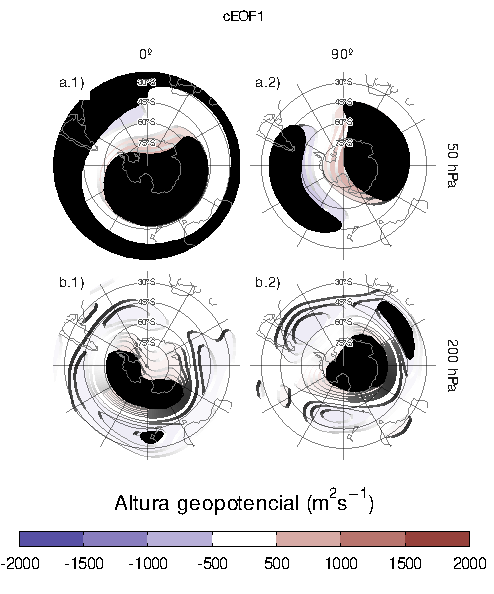
\includegraphics{figures/20-ceofs/eof1-regr-gh-1.pdf}
\caption{\label{fig:eof1-regr-gh}Regresión de anomalías de temperatura geopotencial en SON (\(m^2s^{-1}\)) con la fase 0º (columna 1) y 90º (columna 2) para cEOF1 en 50 hPa (fila a) y 200 hPa (fila b) para el período 1979 -- 2019.
Estos coeficientes fueron obtenidos a partir de una regresión múltiple incluyendo ambas fases.
Áreas con puntos tienen p-valor menor que 0.01 ajustado por FDR.}
\end{figure}
La Figura \ref{fig:eof1-regr-gh} muestra mapas de regresión de anomalías de altura geopotencial en SON sobre el cEOF1.
En 50 hPa (Fig. \ref{fig:eof1-regr-gh} fila a), la fase 0º del cEOF1 está asociada a un centro de anomalías positivas sobre la Antártida con su centro sobre el Mar de Ross.
Por otro lado, el centro de anomalías positivas asociado a la fase 90º está corrido hacia Antártida Oriental y tiene un patrón de onda 1 más evidente.

En 200 hPa (Fig. \ref{fig:eof1-regr-gh} fila b) la fase 0º del cEOF1 muestra un único centro de anomalías positivas que abarca la Antártida Occidental rodeado de anomalías opuestas en latitudes más bajas, con su centro desplazado ligeramente hacia el este en comparación con las anomalías de niveles superiores.
La fase de 90º muestra un patrón mucho más simétrico zonalmente que se asemeja al patrón de anomalías características de la fase negativa del SAM (Fogt and Marshall, 2020).
En ambas fases las anomalías negativas en latitudes bajas son débiles y no son estadísticamente significativas

Por lo tanto, la magnitud y la fase del cEOF1 están asociadas a la magnitud y la fase de una onda zonal principalmente en la estratosfera.


\begin{figure}
\centering
\includegraphics{figures/20-ceofs/eof2-regr-gh-1.pdf}
\caption{\label{fig:eof2-regr-gh}Igual que la Figura \ref{fig:eof1-regr-gh} pero para el cEOF2.}
\end{figure}
La Figura \ref{fig:eof2-regr-gh} muestra los mapas de regresión de las anomalías de altura geopotencial con el cEOF2.
Tanto en 50 como en 200 hPa se observa un patrón de onda 3 similares a los de la Figura \ref{fig:ceofs-1} columna 2.
Las anomalías de regresión asociadas con la fase 0º del cEOF2 están desfasadas 1/4 de longitud de onda con respecto a las asociadas con la fase 90º.
Todos los campos tienen una onda zonal dominante 3 limitada al hemisferio occidental, sobre los océanos Pacífico y Atlántico.

En 50 hPa (Fig. \ref{fig:eof2-regr-gh} fila a) también se ve un monopolo sobre el polo con signo negativo asociado a la fase 0º y signo positivo asociado a la fase 90º.
Este monopolo podría indicar fortalecimiento del vórtice polar asociado a valores positivos del 0º cEOF2 y debilitamiento asociado a valores negativos del 0º cEOF2.
Sin embargo, estas anomalías no son estadísticamente significativas, indicando que su magnitud es baja en comparación a la variabilidad estratosférica y que esta característica no debe sobreinterpretarse.

En 200 hPa (Fig. \ref{fig:eof2-regr-gh} fila b) el tren de ondas es robusto y los centros son estadísticamente significativos, con anomalías insignificantes por fuera de este patrón.
La localización de las anomalías no varía en la vertical, lo cual indica que se trata de un modo barotrópico equivalente.

El cEOF2 representa entonces un tren de ondas barotrópico equivalente muy similar al de los Patrones PSA (Mo and Paegle, 2001).
Comparando la localización de la anomalía positiva cerca de 90ºW en la columna 2 de la Figura \ref{fig:eof2-regr-gh} con las Figuras 1.a y b de Mo and Paegle (2001), el mapa de regresión de la fase 0º podría identificarse con el PSA2, mientras que la fase 90º se asemeja al PSA1.
Estudiaremos la relación entre el cEOF2 y el PSA con más detalle en la Sección \ref{psa}.

\hypertarget{temperatura-y-ozono}{%
\subsubsection{Temperatura y Ozono}\label{temperatura-y-ozono}}


\begin{figure}
\centering
\includegraphics{figures/20-ceofs/eof1-regr-t-1.pdf}
\caption{\label{fig:eof1-regr-t}Igual que la Figura~\ref{fig:eof1-regr-gh} pero para la temperatura del aire (K).}
\end{figure}

\begin{figure}
\centering
\includegraphics{figures/20-ceofs/t-vertical-1.pdf}
\caption{\label{fig:t-vertical}Regresión de anomalías zonales de temperatura (sombrado, Kelvin) y razón de mezcla de ozono (contornos, valores negeativos en línea punteada, etiquetas en partes por mil millón en masa) promediados entre 75°S y 45°S en SON con la fase de 0º (a) y de 90º (b) del cEOF1 para el período 1979 -- 2019.}
\end{figure}
También se evaluó la señal de la variabilidad de los cEOF en la temperatura del aire.
La Figura \ref{fig:eof1-regr-t} muestra los mapas de regresión de las anomalías de la temperatura del aire en 50 hPa y 200 hPa con el cEOF1.
La distribución de los coeficientes de regresión de la temperatura en 50 hPa y en 200 hPa refleja los mapas de regresión de la altura geopotencial en 50 hPa (Fig. \ref{fig:eof1-regr-gh}).
En ambos niveles, la fase de 0º está asociada a anomalías positivas sobre el Polo Sur con su centro desplazado ligeramente hacia 150ºE (Fig. \ref{fig:eof1-regr-t} columna 1).
Por otro lado, los mapas de regresión con la fase de 90º muestran un patrón de onda 1 más claro con su máximo alrededor de los 60ºE.

La Figura \ref{fig:t-vertical} muestra la distribución vertical de los coeficientes de regresión del cEOF1 con las anomalías zonales de la temperatura del aire y de la razón de mezcla de ozono promediadas entre 75°S y 45°S.
Las anomalías zonales de temperatura asociadas al cEOF1 muestran un claro patrón de onda 1 tanto para la fase de 0º como para la de 90º en toda la atmósfera por encima de 250 hPa con una inversión de signo por encima de 10 hPa.
Como resultado del balance hidrostático, este es el nivel en el que la anomalía geopotencial tiene máxima amplitud (no mostrado).

Los valores máximos de la regresión con el ozono coinciden con los valores mínimos de temperatura por encima de 10 hPa y con los máximos por debajo de 10 hPa (Fig. \ref{fig:t-vertical}).
Por tanto, la onda zonal 1 de ozono está correlacionada negativamente con la onda zonal 1 de temperatura en la estratosfera superior, y positivamente en la estratosfera baja.
Este cambio de fase es observado en las anomalías de ozono forzadas por ondas planetarias que alcanzan la estratosfera.
En la estratosfera superior, dominada por procesos fotoquímicos, las temperaturas frías inhiben la destrucción de ozono, explicando el comportamiento opuesto para ambas variables, tal y como se dilucidó con modelos químicos dinámicos (Hartmann and Garcia, 1979; Wirth, 1993; Smith, 1995).
Por otro lado, en la estratosfera baja, dominada por la advección, las anomalías de ozono están desfasadas 1/4 de longitud de onda con el transporte horizontal y vertical, que a su vez están desfasados 1/4 de longitud de onda con las anomalías de temperatura, resultando anomalías del mismo signo para la respuesta de ambas variables (Hartmann and Garcia, 1979; Wirth, 1993; Smith, 1995).




\begin{figure}
\centering
\includegraphics{figures/20-ceofs/o3-regr-1.pdf}
\caption{\label{fig:o3-regr}Regresión de las anomalías de Columna Total de Ozono (CTO, sombreado, unidades Dobson) con la fase 0º (a) y 90º (b) del cEOF1 para el período 1979 -- 2019.
En contornos, la anomalía zonal media de de CTO (contornos negativos en líneas punteadas, unidades Dobson).
Áreas con puntos tienen p-valor menor que 0.01 ajustado por FDR.}
\end{figure}


Los mapas de regresión de las anomalías de CTO con el cEOF1 (Fig. \ref{fig:o3-regr}) muestran patrones de onda zonal 1 asociados a ambas fases del cEOF1.
La posición climatológica del mínimo de ozono durante la primavera (agujero de ozono) no está centrada sobre el Polo Sur, sino que está desplazada hacia el mar de Weddell (p.e., Grytsai, 2011); este desplazamiento se traduce en una onda 1 de la CTO.
Así, el campo de regresión de la fase 0º del cEOF1 (Fig.~\ref{fig:o3-regr}a) coincide con la posición climatológica de esta onda 1 del agujero de ozono, mientras que el campo para la fase 90º está defasado en 90º cEOF1.
La correlación temporal entre la amplitude de la onda 1 de CTO y la amplitud del cEOF1 es 0.77 (CI: 0.61 -- 0.87), mientras que la correlación entre sus fases es -0.84 (CI: -0.91 -- -0.72).
La correlación entre las dos ondas es -0.87 (CI: -0.93 -- -0.77).
Esta relación se muestra en la Figura \ref{fit:wave1-o3}.
En consecuencia, el cEOF1 está fuertemente relacionado con la variabilidad del ozono SH.

\hypertarget{fuentes-de-variabilidad-tropicales}{%
\subsection{Fuentes de variabilidad tropicales}\label{fuentes-de-variabilidad-tropicales}}


\begin{figure}
\centering
\includegraphics{figures/20-ceofs/psi-sst-explained-variance-1.pdf}
\caption{\label{fig:psi-sst-explained-variance}Varianza de la SST (fila a) las anomalías zonales de función corriente (fila b) explicada por el cEOF1 (columna 1) el cEOF2 (columna 2).}
\end{figure}
Para evaluar si la variabilidad de los cEOF analizados está relacionada con fuentes de variabilidad tropicales calculamos la regresión de distintas fases de los cEOFs con las anomalías de SST y con las anomalías zonales de función corriente a 200 hPa.
La Figura \ref{fig:psi-sst-explained-variance} muestra la varianza de cada variable explicada por cada cEOF.

El cEOF1 sólo explica una proporción importante de la varianza de la función corriente al sur de 60º, sugiriendo que no está asociado con la variabilidad tropical.

El cEOF2, en cambio, explica una gran proporción de la variabilidad tropical tanto de la SST como de la función corriente.
Este modo comparte más de un 50\% de la varianza con las SST en el Pacífico central (sugiriendo el impacto del ENSO).
En cuanto a la función corriente, en el Pacífico explica más del 50\% de la varianza en la región del cambio de fecha y sobre Indonesia.
También explica gran parte de la varianza en al oeste y al este de la Península Antártica, llegando a más del 80\% sobre el mar de Amundsen.



\begin{figure}
\centering
\includegraphics{figures/20-ceofs/sst-psi-2-1.pdf}
\caption{\label{fig:sst-psi-2}Regresión de (columan 1) SST (K) y (columna 2) anomalías zonales de función corriente (\(m^2/s\times10^-7\)) y sus vectores de acción de onda con diferentes fases del cEOF2 (indicado con la flecha) en el período 1979 -- 2019.
Áreas con puntos tienen p-valor menor que 0.01 ajustado por FDR.}
\end{figure}
La Figura \ref{fig:sst-psi-2} muestra los mapas de regresión de las anomalías de la temperatura de la superficie del mar (SST) y de la función de corriente a 200 hPa sobre los cEOF2 normalizados.
Además de los mapas de regresión para las fases de 0º y 90º, incluimos las regresiones correspondientes para dos direcciones intermedias (correspondientes a 45º y 135º).

La fase de 90º (fila b) está asociada a fuertes anomalías positivas de la SST en el Pacífico central y oriental y a anomalías negativas en una zona que atraviesa el norte de Australia, Nueva Zelanda y la Zona de Convergencia del Pacífico Sur (SPCZ) (Fig. \ref{fig:sst-psi-2}.b1).
Este patrón es muy similar al patrón del ENSO positivo canónico (Bamston et al., 1997).
De hecho, existe una correlación significativa y muy alta entre el ONI y la serie temporal de la fase de 90º del cEOF2 (0.76 (CI: 0.59 -- 0.87)).
Además del patrón similar al ENSO del Pacífico, también hay anomalías positivas en el océano Índico occidental y valores negativos en el océano Índico oriental, lo que se asemeja a un dipolo del índico en su fase positiva (Saji et al., 1999).
Consistentemente, la correlación entre la fase de 90º del cEOF2 y el DMI es 0.62 (CI: 0.38 -- 0.78).
Sin embargo, la correlación parcial es de 0.32 (p-valor = 0.045), indicando que el DMI explica poca varianza de la fase de 90º del cEOF2 por sí mismo.
Esto puede observarse en la Figura \ref{fig:euler}, donde se ilustra la partición de la varianza de la fase de 90º del cEOF2, el DMI y el ONI.
El DMI aporta, independientemente, sólo un 4.3\% de la varianza mientras que el ONI aporta un 23.8\% por sí mismo.


\begin{figure}
\centering
\includegraphics{figures/20-ceofs/euler-1.pdf}
\caption{\label{fig:euler}(ref:euler-cap)}
\end{figure}
La fase de 90º del cEOF2 está asociado a fuertes anomalías de la función corriente que emanan de los trópicos (Fig. \ref{fig:sst-psi-2}.b2), tanto del sector del Pacífico Central como del Océano Índico.
Esta respuesta atmosférica es consistente con el efecto combinado del ENSO y el DMI sobre los extratropicos: con anomalías de la SST que inducen convección tropical anómala que a su vez excita ondas de Rossby que se propagan meridionalmente hacia latitudes más altas (Mo, 2000; Cai et al., 2011; Nuncio and Yuan, 2015).

Sin embargo, el cEOF2 no está asociado a los mismos patrones de anomalía de las SST tropicales en todas sus fases.
Los paneles d1 y d2 de la Figura \ref{fig:sst-psi-2} muestran que la fase de 0º del cEOF2 no está asociada a ninguna anomalía significativa de las SST ni de la función corriente en los trópicos.
Tampoco la correlación entre el 0º cEOF2 y ENSO es significativa (0 (CI: -0.31 -- 0.3)).
Las filas a y c de la Fig.\ref{fig:sst-psi-2} muestran que las fases intermedias siguen asociadas con anomalías significativas de la SST sobre el Océano Pacífico, pero en lugares ligeramente diferentes.
La fase de 135º está asociada a anomalías de la SST en el Pacífico central (Fig.\ref{fig:sst-psi-2}a.1), mientras que la fase de 45º está asociada a anomalías de la SST que corresponden aproximadamente a los ``sabores'' de ENSO del Pacífico central y del Pacífico oriental, respectivamente (Fig.\ref{fig:sst-psi-2}c.1) (Kao and Yu, 2009).
Ambas fases también están asociadas a trenes de onda que se generan cerca de Australia y se propagan hacia los extratrópicos, aunque menos intensos que los asociados a la fase de 90º.




\begin{figure}
\centering
\includegraphics{figures/20-ceofs/enso-phase-1.pdf}
\caption{\label{fig:enso-phase}Valores del ONI en SON y la fase del cEOF2 en el período 1979 -- 2019.
Los años en los cuales la magnitud del cEOF2 es mayor o menor que la mediana se muestran como diamantes naranja o círculos verdes respectivamente.
La línea negra representa el ajuste ONI \textasciitilde{} sen(fase) computado por cuadrados mínimos pesados por la magnitud del cEOF2.}
\end{figure}
Para explorar la relación entre el forzante tropical y las fases del cEOF2 con más profundidad, la Figura \ref{fig:enso-phase} muestra la relación entre el ONI y la fase del cEOF2 para cada SON entre 1979 y 2019, destacando los años en los que la magnitud del cEOF2 está por encima de la mediana.
En los años con ONI positivo, la fase cEOF2 se sitúa mayoritariamente en torno a la fase de 90º; en los años con ONI negativo, en torno a la fase de -90º.
En las estaciones con ENSO neutro, la fase del cEOF2 es mucho más variable.
La línea negra de la Figura \ref{fig:enso-phase} es un ajuste sinusoidal de la relación entre el ONI y la fase del cEOF2.
El \(r^2\) correspondiente al ajuste es 0.56, estadísticamente significativo con p-valor \textless{} 0.001, lo que indica una relación casi sinusoidal entre estas dos variables.

La correlación entre la magnitud absoluta del ONI y la amplitud del cEOF2 es 0.45 (CI: 0.17 -- 0.67).
Sin embargo, esta relación está determinada principalmente por los tres años con los eventos ENSO más intensos del periodo (2015, 1997, y 1982), los cuales coinciden con los tres años con la magnitud CEOF2 más intensa (no se muestra).
Si se eliminan esos años, la correlación deja de ser significativa (0.05 (CI: -0.28 -- 0.36)).
Además, incluso cuando utilizando todos los años, la correlación de Spearman -que es robusta frente a los valores atípicos- tampoco es significativa (0.2, p-valor = 0.21).
Por lo tanto, aunque la localización de las anomalías tropicales de la SST parece tener un efecto en la definición de la fase del cEOF2, la relación entre la magnitud del cEOF2 y el ONI sigue siendo incierta y podría ser sólo evidente en eventos ENSO muy fuertes, que son escasos en el registro observacional histórico.

Concluimos que el tren de ondas representado por el cEOF2 es tanto parte de la variabilidad interna de la atmósfera extratropical como forzado por las SST tropicales.
En el primer caso, el tren de ondas tiene poca preferencia de fase.
Sin embargo, cuando el cEOF2 es excitado por la variabilidad de la SST tropical, tiende a permanecer fijo en la fase de 90º.



\includegraphics{figures/20-ceofs/sst-psi-1-1.pdf}
La Figura \ref{fig:sst-psi-1} muestra las mismas regresiones que la Figura \ref{fig:sst-psi-2} pero para el cEOF1.
Como anticipó la Figura \ref{fig:psi-sst-explained-variance}, el cEOF1 no está asociado a anomalías significativas de SST ni de función corriente en los trópicos.
En vez de eso, las fases de 0º y 90º están asociadas a flujos de actividad de onda que se propagan zonalmente en los extratópicos cerca de de 60ºS, excepto por un flujo hacia el ecuador desde la costa de la Antártida alrededor de 150ºE en la fase de 0º.
Esto sugiere que la variabilidad de cEOF1 está impulsada principalmente por la variabilidad interna de los extratópicos.

XX HASTA ACÁ XXX

\hypertarget{impactos-en-superficie}{%
\subsection{Impactos en superficie}\label{impactos-en-superficie}}
\begin{figure}
\centering
\includegraphics{figures/20-ceofs/pp-t2m-r2-1.pdf}
\caption{\label{fig:pp-t2m-r2}Explained variance (\(r^2\) as percentage) of 2-metre temperature (row a) and precipitation (row b) anomalies by the regression upon cEOF1 (column 1) and cEOF2 (column 2).}
\end{figure}


También se exploró la influencia de la variabilidad de los cEOF en las anomalías tanto de la temperatura del aire a 2 metros como de la precipitación en el SH.
La Figura \ref{fig:pp-t2m-r2} muestra la varianza explicada de las anomalías de temperatura y precipitación a 2 metros por el modelo lineal múltiple tanto de 0º y 90º cEOF1 (columna 1), como de 0º y 90º cEOF2 (columna 2).
La varianza explicada por cEOF1 para las anomalías de precipitación y las anomalías de temperatura en la mayoría de las regiones es extremadamente baja, excepto para el extremo norte de la Península Antártica, el norte del Mar de Weddell y la costa del Mar de Ross (Fig.\ref{fig:pp-t2m-r2}a.1).

Esta falta de relación fuerte entre el cEOF1 y la SST, la temperatura y la precipitación podría ser sorprendente teniendo en cuenta la correlación entre el cEOF1 y la SAM (Fig. \ref{fig:sam-eof-vertical} columna 1) y la correlación entre la SAM y la SST del Pacífico Central, la temperatura al este y oeste de la Península Antártica, y con la precipitación en el oeste de Australia (Fogt and Marshall, 2020).
Esto se debe principalmente a dos razones.
En primer lugar, la correlación entre cEOF1 y la SAM en la troposfera es modesta, con menos del 50\% de varianza compartida (Fig. \ref{fig:sam-eof-vertical} columna 1), por lo que no se espera que estos índices sean equivalentes.
En segundo lugar, Campitelli et al. (2022) demostró que la fuerte relación entre la SAM y las SST del Pacífico y las anomalías de temperatura alrededor de la Península Antártica se debe principalmente a la parte asimétrica de la SAM.
Mientras tanto, el cEOF1 está significativamente correlacionado sólo con la parte simétrica de la SAM (Fig. \ref{fig:sam-eof-vertical} columna 1), que por sí misma no está significativamente correlacionada con las temperaturas superficiales en esa zona.

Por otro lado, la varianza explicada cEOF2 es superior al 50\% en algunas regiones para ambas variables (Fig.\ref{fig:pp-t2m-r2} columna 2).
Para la temperatura de 2 metros, hay valores altos en el Pacífico tropical y en la SPCZ, así como en la región que sigue un arco entre Nueva Zelanda y el Atlántico Sur, con valores más altos en el Océano Austral.
Sobre los continentes, hay valores moderados de alrededor del 30\% de varianza explicada en el sur de Australia, el sur de Sudamérica y la Península Antártica.
En cuanto a las precipitaciones, los valores son elevados en los trópicos.
En latitudes más altas, se observan valores moderados sobre el este de Australia y algunas regiones del sur de Sudamérica.

Dado que el cEOF1 tiene una señal relativamente débil en las variables de superficie exploradas aquí, sólo nos centraremos en la influencia del cEOF2.
En la Figura \ref{fig:pp-temp-2} se muestran mapas de regresión de las anomalías de temperatura a 2 metros (columna 1) y precipitación (columna 2) sobre diferentes fases del cEOF2 normalizado.


\begin{figure}
\centering
\includegraphics{figures/20-ceofs/pp-temp-2-1.pdf}
\caption{\label{fig:pp-temp-2}Regresión de la temperatura media de 2 metros SON (K, sombreado) y la altura geopotencial de 850 hPa (m, contornos) (columna 1), y la precipitación (correlación, columna 2) sobre diferentes fases de cEOF2. Para el periodo 1979 -- 2019. Las áreas marcadas con puntos tienen valores p inferiores a 0,01 ajustados para la tasa de detección de falsos.}
\end{figure}
Las anomalías de temperatura asociadas a los 90º cEOF (Fig.~\ref{fig:pp-temp-2}.b1) muestran valores positivos en el Pacífico tropical, coherentes con las anomalías de SST asociadas a la misma fase (Fig.~\ref{fig:sst-psi-2}.b1).
En latitudes más altas existe un patrón ondulatorio de valores positivos y negativos que coincide con los nodos de los patrones de regresión de la altura geopotencial de 850 hPa.
Esto es coherente con las anomalías de temperatura producidas por la advección meridional de temperatura por los vientos meridionales derivados del equilibrio geostrófico.
Sobre los continentes, el 90º cEOF2 (Fig.\ref{fig:pp-temp-2}b.1) se asocia con anomalías de temperatura de regresión positiva en el sur de Australia y anomalías de regresión negativa en el sur de Sudamérica y la Península Antártica, que son resultado del tren de ondas descrito anteriormente.

Las anomalías de temperatura asociadas al 0º cEOF2 (Fig.\ref{fig:pp-temp-2}d.1) son menos extensas y se limitan a latitudes medias y altas.

Sobre los continentes, las regresiones de las anomalías de temperatura no son significativas, excepto las anomalías positivas cerca de la Península Antártica.

Las anomalías de precipitación tropical asociadas con el 90º cEOF2 son fuertes, con anomalías positivas en el Pacífico central y el Índico occidental, y anomalías negativas en el Pacífico oriental (Fig.\ref{fig:pp-temp-2}b.2).
Este campo es consistente con el mapa de regresión de la SST (Fig.\ref{fig:pp-temp-2}b.1) ya que las anomalías positivas de la SST potencian la convección tropical y las anomalías negativas de la SST la inhiben.

En los extratropicales, el 90º cEOF2 positivo está relacionado con condiciones más secas sobre el este de Australia y el océano circundante, que es una señal similar a la asociada con ENSO (Cai et al., 2011).
Sin embargo, el 90º cEOF2 no es la fase más correlacionada con las precipitaciones en esa zona.
La componente de la fase 135º (una intermedia entre las positivas de 90º y 180º cEOF2) está asociada con correlaciones temporales más fuertes y extensas con la precipitación sobre Australia y Nueva Zelanda.
La influencia del cEOF2 en la precipitación australiana podría estar más relacionada con los impactos directos de las anomalías de la SST en los océanos circundantes que en el patrón de interconexión representado por el cEOF2.

Sobre Sudamérica, el 90º cEOF2 tiene correlaciones positivas con la precipitación en el sudeste de Sudamérica (SESA) y el centro de Chile, y correlaciones negativas en el este de Brasil.
Este campo de correlación coincide con la firma de precipitación primaveral de ENSO (e.g. Cai et al., 2020) y también es similar a las anomalías de precipitación asociadas con el A-SAM (Campitelli et al., 2022).
Este resultado no es sorprendente teniendo en cuenta la estrecha relación del 90º cEOF2 tanto con el ONI como con el índice A-SAM, demostrada anteriormente.
Además, consolida la identificación del cEOF2 con el patrón PSA.
Semejante a la relación entre ONI y la fase de cEOF2 (Fig. \ref{fig:enso-phase}), existe una dependencia de fase de cEOF2 de las anomalías de precipitación en SESA (no mostrado).

Los coeficientes de correlación entre las anomalías de precipitación y el 0º cEOF2 (Fig.~\ref{fig:pp-temp-2}d.2) son más débiles que para 90º cEOF2.
Hay una correlación positiva residual en el Pacífico oriental ecuatorial y pequeñas correlaciones positivas, no estadísticamente significativas, sobre el este de Australia y negativas sobre Nueva Zelanda.

\hypertarget{otras-estaciones}{%
\section{Otras estaciones ??}\label{otras-estaciones}}

Definitivamente extender al resto del año.
(índice mensual).
Esto faltaría.
Hay código para hacerlo, pero falta la interpretación, que es lo importante.

Sería un análisis más modesto.

\hypertarget{estructura-simuxe9trica-y-asimuxe9trica-del-sam}{%
\chapter{Estructura simétrica y asimétrica del SAM}\label{estructura-simuxe9trica-y-asimuxe9trica-del-sam}}

\hypertarget{introducciuxf3n-1}{%
\section{Introducción}\label{introducciuxf3n-1}}

El Modo Anular Austral (SAM) es el principal modo de variabilidad de la circulación extratropical del hemisferio sur (Rogers and van Loon, 1982) en escalas temporales diarias, mensuales y decenales (Baldwin and Dunkerton, 2001; Fogt and Bromwich, 2006) y ejerce una importante influencia en las anomalías de temperatura y precipitación, así como en la concentración de hielo marino (p.~ej. Fogt and Marshall, 2020).
Su fase positiva suele describirse como presiones anómalamente bajas sobre la Antártida rodeadas de un anillo de altas presiones anómalas en latitudes medias y altas.

La mayoría de los autores describen el SAM como un patrón zonalmente simétrico, hecho que se refleja no sólo en su nombre, sino también en los diversos métodos utilizados para caracterizarlo.
De los distintos índices presentados en la literatura, muchos de ellos se basan en medias zonales de la presión a nivel del mar o de la altura geopotencial (Ho et al., 2012).
Gong and Wang (1999) definió el índice SAM como la diferencia de presión media zonal a nivel del mar entre 40\degree S y 65\degree S, que es también la definición utilizada por el índice basado en estaciones de Marshall (2003).
Baldwin and Thompson (2009) propuso definir los modos anular septentrional y meridional como la EOF principal de la altura geopotencial promediada zonalmente en cada nivel.

Aunque estos índices se basan en promedios zonales, sus anomalías espaciales de altura geopotencial asociadas contienen notables desviaciones de la simetría zonal, particularmente en la región del Océano Pacífico.
Las asimetrías zonales no han sido ampliamente estudiadas, pero trabajos previos sugieren que modulan fuertemente los impactos regionales de la SAM (Fan, 2007; Silvestri and Vera, 2009; Fogt et al., 2012; Rosso et al., 2018).
El hecho de que la SAM no sea totalmente simétrica zonalmente dificulta nuestra capacidad para reconstruir su variabilidad histórica antes de la disponibilidad de observaciones densas en el hemisferio sur (Jones et al., 2009).

Parte de la variabilidad asociada a las asimetrías zonales de la SAM parece estar forzada por los trópicos.
La variabilidad de tipo ENOS afecta a los extratópicos del Hemisferio Sur a través de los trenes de ondas de Rossby (Mo and Ghil, 1987; Kidson, 1988; Karoly, 1989) que se proyectan fuertemente sobre las anomalías zonales asociadas a la SAM en el sector del Pacífico.
Además, se han observado influencias tropicales en la SAM (Fan, 2007; Fogt et al., 2011; Clem and Fogt, 2013).
Fan (2007) calculó los índices de SAM de los hemisferios occidental y oriental por separado y descubrió que estaban mucho más correlacionados entre sí si se eliminaba la señal (lineal) del ENSO.

Varios investigadores han documentado tendencias positivas en la SAM utilizando diferentes índices, sobre todo en verano y otoño austral (por ejemplo, Fogt and Marshall, 2020 y sus referencias).
Se cree que estas tendencias están impulsadas principalmente por el agotamiento del ozono estratosférico y el aumento de los gases de efecto invernadero, y se entienden en el contexto de las variables medias zonales (Marshall et al., 2004; Gillett et al., 2005; Arblaster and Meehl, 2006; Gillett et al., 2013).
Sin embargo, aún no está claro cómo o si el componente SAM asimétrico responde a estos forzamientos, o cómo su variabilidad altera las tendencias observadas.

El impacto de la componente zonalmente asimétrica de la SAM a escala regional aún no se ha estudiado en detalle.
La fase positiva de la SAM se asocia con temperaturas más frías de lo normal sobre la Antártida y más cálidas de lo normal en latitudes más bajas (Jones et al., 2019) (y viceversa para la SAM negativa).
Pero hay desviaciones significativas de esta respuesta media zonal, especialmente en la Península Antártica y el Atlántico sur (Fogt et al., 2012).
La señal relacionada con SAM en las anomalías de precipitación se comporta de forma similar, aunque con una desviación aún mayor de la simetría zonal (Lim et al., 2016).
La relación SAM-precipitación en el sudeste de Sudamérica puede explicarse por la circulación zonalmente asimétrica similar a la del Pacífico-Sudamérica (PSA) asociada a la SAM (Silvestri and Vera, 2009; Rosso et al., 2018).
Fan (2007) también descubrió que las precipitaciones en Asia oriental se veían afectadas por la variabilidad de la parte occidental de la SAM.

El estudio de la variabilidad temporal del componente asimétrico de la SAM no ha recibido mucha atención, excepto por Fogt et al. (2012).
Este estudio aporta evidencias sobre la relevancia del componente asimétrico de la SAM.
Sin embargo, sus conclusiones se basan en composiciones de eventos SAM positivos y negativos que incluyen un pequeño número de casos desigualmente distribuidos entre años con y sin información satelital.
Esto último es especialmente importante debido a las inhomogeneidades en los productos de reanálisis anteriores a la era de los satélites y al posible cambio en la estructura asimétrica de la SAM (Silvestri and Vera, 2009).
Además, Fogt et al. (2012) estudió la componente asimétrica zonal de la SAM sólo en la presión a nivel del mar.
Las asimetrías zonales en el patrón espacial de la SAM son bastante barotrópicas en toda la troposfera, pero cambian drásticamente en la estratosfera (Baldwin and Thompson, 2009).

En resumen, las investigaciones previas sugieren fuertemente que el componente zonalmente asimétrico de la SAM puede ser potencialmente muy diferente del componente zonalmente simétrico.
Podría tener diferentes fuentes de variabilidad, impactos y respuesta a largo plazo al forzamiento radiativo.
Un único índice SAM que mezcle la variabilidad zonalmente simétrica y zonalmente asimétrica sólo es capaz de captar el efecto combinado de estos dos modos potencialmente distintos.

Nuestro objetivo es, por tanto, describir los componentes zonalmente asimétricos y simétricos de la variabilidad de la SAM.
En primer lugar, proponemos una metodología que proporciona, para cada nivel, dos índices que pretenden captar de forma independiente la variabilidad del componente SAM simétrico y asimétrico, respectivamente.
En consecuencia, se evalúan su estructura vertical y su coherencia, así como su variabilidad temporal y sus tendencias.
A continuación se estudian los patrones espaciales descritos por la variabilidad exclusiva de cada índice centrándose en 50 hPa como representación de la estratosfera y 700 hPa como representación de la troposfera.
Por último, se investigan las relaciones de la SAM a 700 hPa con las anomalías de temperatura y precipitación.

\hypertarget{datos-y-muxe9todos-1}{%
\section{Datos y métodos}\label{datos-y-muxe9todos-1}}

\hypertarget{definiciuxf3n-de-los-uxedndices}{%
\subsection{Definición de los índices}\label{definiciuxf3n-de-los-uxedndices}}

Tradicionalmente, la SAM se define como el modo ortogonal empírico (EOF) principal de las anomalías de la presión al nivel del mar o de la altura geopotencial en niveles bajos (Ho et al., 2012).
Siguiendo a Baldwin (2001), ampliamos esa definición verticalmente y utilizamos el término SAM para referirnos al EOF principal de las anomalías mensuales de la altura geopotencial al sur de 20 grados S en cada nivel.
Realizamos EOFs calculando la Descomposición de Valor Singular de la matriz de datos consistente en 489 filas y 4176 columnas (144 puntos de longitud y 29 puntos de latitud).
Ponderamos los valores por la raíz cuadrada del coseno de la latitud para tener en cuenta el área no igual de cada punto de cuadrícula (Chung and Nigam, 1999).
En el análisis EOF consideramos todos los meses juntos sin dividir por estaciones.

Para separar los componentes zonalmente simétricos y asimétricos de la SAM, calculamos la media zonal y las anomalías del patrón espacial completo de la SAM, como se muestra en la Figura \ref{fig:method} a 700 hPa.
La señal espacial completa (\(\mathrm{EOF_1}(\lambda, \phi)\)) es la suma de los componentes zonalmente asimétricos (\(\mathrm{EOF_1^*}(\lambda, \phi)\)) y simétricos (\([\mathrm{EOF_1}](\lambda, \phi)\)).
A continuación, calculamos el índice SAM, el índice SAM asimétrico (A\nobreakdash-SAM) y los índices SAM simétrico (S\nobreakdash-SAM) como los coeficientes de la regresión de cada campo de altura geopotencial mensual sobre los respectivos patrones (ponderando por el coseno de la latitud).
A continuación, los tres índices se normalizan dividiéndolos por la desviación típica del índice SAM en cada nivel.
Como resultado, las magnitudes entre los índices son comparables.
Sin embargo, sólo el índice SAM tiene desviación típica unitaria por definición.
La varianza explicada de cada patrón se utiliza como indicador del grado de simetría o asimetría zonal de cada campo mensual.
Para cuantificar la coherencia entre las series temporales correspondientes a distintos índices o al mismo índice en distintos niveles, calculamos la correlación temporal entre ellas.


\begin{figure}
\centering
\includegraphics{figures/30-sam/method-1.pdf}
\caption{\label{fig:method}Spatial patterns of the first EOF of 700~hPa geopotential height for 1979 -- 2018 period1. (a) Full field, (b) zonally asymmetric component and (c) zonally symmetric component. Arbitrary units; positive values in blue and negative values in red.}
\end{figure}
El método supone la linealidad de la componente asimétrica de la SAM.
Esto significa que las asimetrías zonales asociadas a la fase positiva de SAM (SAM+) son de signo casi opuesto y de la misma magnitud que las asociadas a la fase negativa de SAM (SAM-).
Las composiciones de Fogt et al. (2012) (su Figura 4) sugieren que esto podría no ser del todo válido, aunque gran parte de esa aparente no linealidad podría deberse a la naturaleza heterogénea de los años seleccionados para construir las composiciones.
Para probar esta suposición, calculamos compuestos estacionales de anomalías zonales de altura geopotencial para SAM+ y SAM- (definidos como meses en los que el índice SAM es mayor que 1 desviación estándar y menor que menos 1 desviación estándar, respectivamente) para el periodo de 1979 a 2018 en los niveles de 700 hPa y 50 hPa (Figuras \ref{fig:A3} y \ref{fig:A4}).
En todas las estaciones y en ambos niveles, los compuestos SAM+ son similares a los SAM- en estructura pero con signo opuesto.
Las correlaciones espaciales entre los compuestos de cada estación son elevadas.
El método considerado en este estudio parece entonces una aproximación razonable del fenómeno.

Al realizar el análisis EOF utilizando los datos de todos los meses estamos asumiendo que la estructura zonalmente asimétrica de la SAM es la misma en todas las estaciones.
Esto último se evaluó calculando las anomalías zonales de la altura geopotencial mediante la proyección de la primera EOF de cada estación de forma independiente.
Se consideraron las siguientes estaciones: diciembre a febrero (DJF), marzo a mayo (MAM), junio a agosto (JJA) y septiembre a noviembre (SON).
Los resultados son muy similares entre sí en la troposfera (Figura \ref{fig:A5}, fila 2) y muestran correlaciones espaciales entre 0,65 (DJF con JJA) y 0,9 (MAM con SON).
En la estratosfera (Figura \ref{fig:A5}, fila 1), los patrones son similares para todas las estaciones excepto DJF, cuando las anomalías zonales de la onda-1 se giran 90\degree en comparación con el resto del año.
Las correlaciones espaciales en la estratosfera se sitúan entre -0,24 (DJF con SON) y 0,95 (MAM con JJA).
Por tanto, los resultados confirman que la estructura asimétrica zonal de la SAM es muy similar durante la mayor parte del año.
El trimestre DJF muestra correlaciones mucho más bajas con las otras estaciones en ambos niveles y las anomalías zonales más débiles (Figura \ref{fig:A3}), lo que concuerda con Fogt and Marshall (2020).
Por tanto, cabría esperar que, aunque el análisis se realice incluyendo todos los meses, represente con mayor precisión el resto de las estaciones.

El método también asume que el patrón zonalmente asimétrico de la SAM permanece estacionario a lo largo del periodo considerado.
Silvestri and Vera (2009) sugieren que este podría no ser el caso entre 1958 y 2004.
Los patrones asimétricos zonales de SAM se calcularon para las dos mitades del periodo (1979 a 1998 y 1999 a 2018) respectivamente.
Las diferencias entre los dos periodos parecen ser relativamente pequeñas tanto en la troposfera como en la estratosfera (Figura \ref{fig:A6}).

\hypertarget{regresiones}{%
\subsection{Regresiones}\label{regresiones}}

Realizamos regresiones lineales para cuantificar la asociación entre los índices SAM y otras variables.
Además, aplicamos un análisis de regresión lineal múltiple para describir la influencia combinada de A\nobreakdash-SAM y S\nobreakdash-SAM.
Para obtener los coeficientes lineales de una variable \(X\) (geopotencial, temperatura, precipitación, etc\ldots) con A\nobreakdash-SAM y S\nobreakdash-SAM ajustamos la ecuación

\[
X(\lambda, \phi, t) = \alpha(\lambda, \phi) \operatorname{A-SAM} + \beta(\lambda, \phi) \operatorname{S-SAM} + X_0(\lambda, \phi) + \epsilon(\lambda, \phi, t)
\]

donde \(\lambda\) y \(\phi\) son la longitud y la latitud, \(t\) es el tiempo, \(\alpha\) y \(\beta\) son los coeficientes de regresión lineal, \(X_0\) y \(\epsilon\) son la constante y los términos de error.
A partir de esta ecuación, \(\alpha\) representa la asociación (lineal) de \(X\) con la variabilidad de A\nobreakdash-SAM que no se explica por la variabilidad de S\nobreakdash-SAM; es decir, es proporcional a la correlación parcial de \(X\) y A\nobreakdash-SAM, controlando el efecto de S\nobreakdash-SAM, y viceversa para \(\beta\).
Al realizar una regresión separada para cada trimestre (DJF, MAM, JJA, SON), promediamos estacionalmente las variables relevantes para cada año y trimestre antes de calcular la regresión.

La significación estadística de los campos de regresión se evaluó ajustando los valores p mediante el control de la Tasa de Falsos Descubrimientos (Benjamini and Hochberg, 1995; Wilks, 2016) para evitar resultados engañosos derivados del elevado número de regresiones (Walker, 1914; Katz and Brown, 1991).

Las tendencias lineales se calcularon mediante mínimos cuadrados ordinarios y el intervalo de confianza del 95\% se calculó asumiendo una distribución t con los grados de libertad residuales apropiados.
La amplitud de las ondas zonales se define calculando la transformada de Fourier del campo espacial en cada círculo de latitud.

Calculamos las estimaciones de probabilidad de densidad utilizando un kernel gaussiano de anchura óptima según Sheather and Jones (1991).

\hypertarget{resultados}{%
\section{Resultados}\label{resultados}}

\hypertarget{temporal}{%
\section{Temporal evolution}\label{temporal}}
\begin{figure}
\centering
\includegraphics{figures/30-sam/asymsam-timeseries-1.pdf}
\caption{\label{fig:asymsam-timeseries}Time series for A-SAM and S-SAM at (a) 50\textasciitilde hPa and (b) 700\textasciitilde hPa. To the right, probability density estimate of each index. Series are standardised by the standard deviation of the SAM at each level.}
\end{figure}
En primer lugar, evaluamos la evolución temporal de A\nobreakdash-SAM y S\nobreakdash-SAM.
La figura \ref{fig:asymsam-timeseries} muestra las series temporales correspondientes para 700 hPa y 50 hPa y sus correspondientes estimaciones de densidad.
Seleccionamos estos dos niveles como representativos de la variabilidad troposférica y estratosférica respectivamente.
Como se muestra a continuación, las variabilidades de ambos índices son muy coherentes dentro de cada capa atmosférica, por lo que es razonable tomar un nivel como representativo de cada capa.

La variabilidad mes a mes es evidente para ambos índices, con variaciones ruidosas en las frecuencias bajas.
A primera vista, las series pueden distinguirse por sus distribuciones.
En comparación con los índices troposféricos, los estratosféricos son mucho más de cola larga; es decir, abundan los valores extremos (tanto negativos como positivos).
Las series A\nobreakdash-SAM tienen a la vez más variabilidad en las frecuencias más altas que las series S\nobreakdash-SAM.

El S\nobreakdash-SAM estratosférico varía fuertemente con un periodo entre 15 y 30 meses (el espectro máximo se sitúa en 12 meses), lo que puede apreciarse mediante el análisis espectral (Figura \ref{fig:A2}).
En el periodograma del S\nobreakdash-SAM troposférico se aprecia un pico local en un rango de frecuencias similar, aunque no es estadísticamente significativo.
Esta banda de periodicidad está alrededor del rango de periodicidad de la Oscilación Cuasi-Bienal (Baldwin et al., 2001) y es consistente con (Vasconcellos et al., 2022), quien encontró que la SAM y la QBO comparten una alta potencia común significativa alrededor de la banda de 2 años.
El hecho de que esta periodicidad no sea evidente en el índice A\nobreakdash-SAM, también es consistente con sus composiciones de anomalías de altura geopotencial durante la QBO oriental y occidental, que muestran un monopolo bastante simétrico sobre la Antártida.
En la troposfera, el pico de variabilidad más significativo se encuentra en A\nobreakdash-SAM en torno a 36 meses.

En una inspección visual, las series temporales A\nobreakdash-SAM y S\nobreakdash-SAM parecen estar correlacionadas.
Además, observando los extremos en la estratosfera, la serie S\nobreakdash-SAM parece ir por detrás de la serie A\nobreakdash-SAM (véanse, por ejemplo, los eventos positivos de finales de 1987).
La figura \ref{fig:cor-lev} muestra estas correlaciones a lo largo de todos los niveles considerados, para los retardos cero y -1.
Los valores de las correlaciones de retardo cero entre A\nobreakdash-SAM y S\nobreakdash-SAM son relativamente constantes en toda la troposfera, fluctuando entre 0.32 y 0.4.
Las correlaciones con desfase de un mes son igualmente constantes, pero se reducen significativamente a alrededor de 0.13.
En la estratosfera, las correlaciones de desfase cero caen a un mínimo de 0.14 en 20 hPa y luego aumentan de nuevo monotónicamente con la altura hasta el nivel más alto del reanálisis (aunque los resultados cerca de la parte superior de los modelos deben interpretarse con cuidado).
Al mismo tiempo, las correlaciones de un mes de retraso aumentan con la altura.
Por lo tanto, el índice A\nobreakdash-SAM estratosférico tiende a preceder al índice S\nobreakdash-SAM.
(Las correlaciones en los desfases de -5 a 5 se muestran en la Figura \ref{fig:A1}).
\begin{figure}
\centering
\includegraphics{figures/30-sam/cor-lev-1.pdf}
\caption{\label{fig:cor-lev}Correlation between S-SAM and A-SAM at each level for lag zero and lag -1 (A-SAM leads S-SAM) for the 1979 -- 2018 period.}
\end{figure}
\begin{figure}
\centering
\includegraphics{figures/30-sam/cross-correlation-1.pdf}
\caption{\label{fig:cross-correlation}Cross correlation between levels for the (a) SAM, (b) A-SAM, and (c) S-SAM for the 1979 -- 2018 period.}
\end{figure}
La figura \ref{fig:cross-correlation} muestra la correlación cruzada (lag cero) entre niveles para los índices SAM, A\nobreakdash-SAM y S\nobreakdash-SAM.
Para el SAM (Figura \ref{fig:cross-correlation}a), los valores altos por debajo de 100 hPa reflejan la coherencia vertical (lag cero) en toda la troposfera.
Por encima de 100 hPa, la correlación entre niveles disminuye más rápidamente, lo que indica una variabilidad menos coherente (desfase cero).
Sin embargo, las correlaciones entre los niveles troposféricos y los niveles estratosféricos bajos y medios siguen siendo relativamente altas (por ejemplo, más de 0,4 entre los niveles troposféricos y los niveles por debajo de 30 hPa).
A\nobreakdash-SAM y S\nobreakdash-SAM (Figura \ref{fig:cross-correlation}b y c, respectivamente) comparten un alto nivel de coherencia similar en la troposfera, pero difieren en su comportamiento estratosférico.
La coherencia estratosférica es mayor para el A\nobreakdash-SAM que para el S\nobreakdash-SAM.
La S\nobreakdash-SAM estratosférica parece conectarse con más fuerza a la troposfera que la A\nobreakdash-SAM estratosférica.
\begin{figure}
\centering
\includegraphics{figures/30-sam/trends-1.pdf}
\caption{\label{fig:trends}Linear trends (in standard deviations per decade) at each level for annual (row 1) and seasonal values (rows 2 to 5) for the period 1979 -- 2018 and for the (column a) SAM index, (column b) A-SAM index, and (column c) S-SAM index. Shading indicates the 95 confidence interval from a t-distribution.}
\end{figure}
Las tendencias lineales para cada uno de los índices (SAM, S\nobreakdash-SAM y A\nobreakdash-SAM) se evaluaron para el periodo completo 1979 -- 2018 en cada nivel para el año completo y separado por trimestres (Figura \ref{fig:trends}).
El índice SAM presenta una tendencia significativa estadísticamente positiva (Figura \ref{fig:trends}b.1) que se extiende por toda la troposfera hasta aproximadamente 50 hPa y alcanza su valor máximo a 100 hPa.
Las tendencias estacionales (resto de la Figura \ref{fig:trends} columna a) indican que las tendencias positivas están presentes en otoño y sobre todo en verano, donde el máximo de 100 hPa está mucho más definido.
En invierno y primavera, no detectamos ninguna tendencia estadísticamente significativa.
Esto es coherente con los resultados de estudios anteriores, que encuentran grandes tendencias positivas en verano, menores en otoño y ninguna tendencia en las demás estaciones (por ejemplo, Fogt and Marshall (2020) y referencias en él) utilizando índices de la SAM basados en la circulación en superficie o cerca de la superficie.

Al separar la señal SAM en sus partes asimétrica y simétrica, no sólo podemos ver que estas tendencias se deben casi por completo al componente simétrico (columna b frente a columna c en la Figura \ref{fig:trends}), sino que en algunos casos las tendencias se vuelven más claras.
En verano, A\nobreakdash-SAM tiene una tendencia negativa estadísticamente no significativa en la troposfera media que oculta la tendencia en el índice SAM; como resultado, las tendencias calculadas utilizando sólo el componente simétrico son más fuertes (comparar la región sombreada en la Figura \ref{fig:trends}b.2 y c.2).
En otoño, el índice S\nobreakdash-SAM revela una tendencia positiva estadísticamente significativa en la estratosfera que no es significativa utilizando el índice SAM.

Una tendencia positiva en el índice S\nobreakdash-SAM y ninguna tendencia en el índice A\nobreakdash-SAM podría sugerir en un primer momento una tendencia hacia una SAM más simétrica.
Sin embargo, un S\nobreakdash-SAM muy negativo con tendencia a un S\nobreakdash-SAM menos negativo se traduciría en una tendencia positiva del S\nobreakdash-SAM pero en una SAM más asimétrica.
\begin{figure}
\centering
\includegraphics{figures/30-sam/r-squared-trend-1.pdf}
\caption{\label{fig:r-squared-trend}Linear trends (in percent per decade) of the variance explained by A-SAM and S-SAM at each level and for each trimester for the period 1979 -- 2018. Shading indicates the 95 confidence interval.}
\end{figure}
aaa
Para estudiar la cuestión de si la SAM se está volviendo más o menos asimétrica, mostramos las tendencias de la varianza explicada de cada índice para cada trimestre en la Figura \ref{fig:r-squared-trend}.
En la troposfera, la única tendencia significativa es la de DJF, en la que el A\nobreakdash-SAM tiene una tendencia positiva de alrededor del 2\% por década, lo que sugiere que el DJF SAM se ha vuelto más asimétrico en el período de 1979 a 2018.
Fogt et al. (2012) observó un cambio de una SAM más asimétrica antes de 1980 a una SAM más simétrica después de 1980, pero nuestro periodo de estudio (1979 -- 2018) nos impide detectar ese cambio.
Sin embargo, debido a la naturaleza atípica del componente asimétrico de la SAM durante la DJF (Sección \ref{definition-of-indices}), esto debe tomarse sólo como una evidencia preliminar.
La otra tendencia significativa se da en la estratosfera durante SON, donde hay una tendencia positiva en la varianza explicada por la S\nobreakdash-SAM de aproximadamente un 4\% por década.
Este cambio podría ser el resultado del forzamiento provocado por el agotamiento del ozono.

\hypertarget{spatial}{%
\section{Spatial patterns}\label{spatial}}
\begin{figure}
\centering
\includegraphics{figures/30-sam/2d-regr-1.pdf}
\caption{\label{fig:2d-regr}Regression of geopotential height (meters) at (row 1) 50\textasciitilde hPa and (row 2) 700\textasciitilde hPa with (column a) SAM, (column b) A-SAM, and (column c) S-SAM for the 1979 -- 2018 period4. The regression patterns for A-SAM and S-SAM are the result of one multiple regression using both indices. Points marked on panel b.2 are the location of the reference points used by \cite{raphael2004} for their Zonal Wave 3 index.}
\end{figure}
A continuación calculamos la regresión espacial de las anomalías de altura geopotencial sobre los índices A\nobreakdash-SAM y S\nobreakdash-SAM en los niveles de 700 hPa y 50 hPa (Figura \ref{fig:2d-regr}).
Mientras que los coeficientes de regresión de la columna a de la Figura \ref{fig:2d-regr} se calculan utilizando SAM, los coeficientes de regresión de las columnas b y c de la Figura \ref{fig:2d-regr} se calculan mediante regresión múltiple utilizando los índices A\nobreakdash-SAM y S\nobreakdash-SAM al mismo tiempo.
Así, deben interpretarse como los patrones asociados a cada índice, eliminando la variabilidad (linealmente) explicada por el otro.

En la estratosfera, el patrón espacial asociado al SAM está claramente dominado por una estructura zonalmente simétrica y monopolar (Figura \ref{fig:2d-regr}a.1) que no está centrada en el Polo Sur.
Por otro lado, el monopolo asociado a S\nobreakdash-SAM (Figura \ref{fig:2d-regr}c.1) es más simétrico, aunque sigue sin estar perfectamente centrado en el Polo Sur.
Además, el patrón de regresión de A\nobreakdash-SAM se caracteriza por una estructura de onda-1 con centros sobre el Pasaje de Drake en el Hemisferio Occidental y el Mar de Davis en el Hemisferio Oriental.

En la troposfera, el patrón de regresión asociado al SAM muestra la conocida combinación de modo anular zonalmente simétrico con asimetrías zonales en forma de onda-3 (Figura \ref{fig:2d-regr}a.2, (Fogt et al., 2012)).
Los patrones de regresión asociados a los índices A\nobreakdash-SAM y S\nobreakdash-SAM desentrañan con éxito ambas estructuras.
Obsérvese que, a la luz del debate anterior sobre la naturaleza atípica de la DJF, es probable que este efecto medio anual no represente perfectamente la DJF.
Mientras que el índice A\nobreakdash-SAM da lugar a una onda zonal más limpia (Figura \ref{fig:2d-regr}b.2), el índice S\nobreakdash-SAM se asocia a una estructura anular, con sólo asimetrías zonales vestigiales (Figura \ref{fig:2d-regr}c.2) en forma de una onda-3 que es la inversa de la onda-3 A\nobreakdash-SAM.
El patrón de onda-3 observado en la figura \ref{fig:2d-regr}b.2 está girado media longitud de onda respecto a la posición media del patrón de onda-3 medio descrito por Raphael (2004), cuyas posiciones de referencia están marcadas con puntos en la figura.
De hecho, no existe correlación entre el índice de Raphael (2004) y A\nobreakdash-SAM (cor = -0.14, p-value \textless{} 0.001).
Así, el índice A\nobreakdash-SAM troposférico representa un desplazamiento zonal en la posición del patrón climatológico de la onda-3.


\begin{figure}
\centering
\includegraphics{figures/30-sam/wave-amplitude-1.pdf}
\caption{\label{fig:wave-amplitude}Amplitud (metros) de las ondas zonales de los patrones de regresión de altura geopotencial de la Figura \ref{fig:2d-regr} para ondas zonales con número de onda 0, 1, 2 y 3, donde el número de onda 0 representa la amplitud de la media zonal.}
\end{figure}
La amplitud de los primeros números de onda zonales en cada latitud a 50 hPa y 700 hPa se muestran en la Figura \ref{fig:wave-amplitude}, donde el número de onda cero representa la amplitud de la media zonal.
Las amplitudes de las ondas zonales del patrón espacial descrito por el índice SAM (Figura \ref{fig:wave-amplitude} columna a) están dominadas por la media zonal (número de onda 0) en ambos niveles.
Sin embargo, las ondas zonales son importantes, sobre todo al sur de 50 grados S, con un número de onda 1 claramente dominante a 50 hPa (Figura \ref{fig:wave-amplitude}a.1) y una mezcla de ondas de amplitud similar a 700 hPa (Figura \ref{fig:wave-amplitude}a.2).
La figura \ref{fig:wave-amplitude} columna b muestra que el A\nobreakdash-SAM está abrumadoramente dominado por la onda 1 en la estratosfera (Figura @ref(fig: onda-amplitud)b.1), mientras que en la troposfera se explica por una combinación de ondas zonales 3 a 1 en nivel decreciente de importancia (Figura \ref{fig:onda-amplitud}b.2) con una amplitud despreciable de la media zonal.
Por otra parte, el S\nobreakdash-SAM se explica casi en su totalidad por la media zonal en ambos niveles (Figura \ref{fig:wave-amplitude} columna c), con poca o ninguna contribución de las ondas zonales con números de onda de 1 a 3.
\begin{figure}
\centering
\includegraphics{figures/30-sam/vertical-regression-1.pdf}
\caption{\label{fig:vertical-regression}Regression between monthly geopotential height anomalies (meters) averaged betweeen 65 and 40 S and the A-SAM index (extracted from a multiple regression which included the S-SAM index). (a) With the A-SAM in 50\textasciitilde hPa and (b) in 700\textasciitilde hPa for the 1979 -- 2018 period5.}
\end{figure}
Para analizar la estructura vertical de las anomalías de altura geopotencial asociadas al índice A\nobreakdash-SAM, mostramos una sección transversal vertical de regresiones de altura geopotencial media entre 65\degree S y 40\degree S para el índice A\nobreakdash-SAM de 50 hPa (Figura \ref{fig:vertical-regression}a) y para el índice A\nobreakdash-SAM de 700 hPa (Figura \ref{fig:vertical-regression}b).
Las anomalías de altura geopotencial asociadas a la A\nobreakdash-SAM estratosférica (Figura \ref{fig:vertical-regression}a) están claramente limitadas a la estratosfera, lo que subraya el desacoplamiento entre la A\nobreakdash-SAM estratosférica y la troposférica.
La estructura vertical de esta señal se inclina unos 60 grados hacia el oeste entre 100 hPa y 1 hPa, lo que sugiere procesos baroclínicos.
La señal en la estratosfera se maximiza cerca de 10 hPa a pesar de utilizar el índice de 50 hPa para la regresión.

El A\nobreakdash-SAM troposférico (Figura \ref{fig:vertical-regression}b) presenta señales significativas que se extienden hacia arriba hasta los niveles superiores considerados.
En la troposfera, la estructura de la onda 3 es barotrópica equivalente, con una amplitud máxima en torno a los 250 hPa.
Las anomalías son mayores en el hemisferio occidental, donde se extienden hasta la estratosfera.
En el hemisferio oriental, la señal de la onda 3 es menor y se limita a la troposfera, mientras que las anomalías negativas dominan en la estratosfera.
Así, mientras que el índice A\nobreakdash-SAM troposférico está asociado a anomalías geopotenciales estratosféricas, éstas no se proyectan fuertemente sobre el A\nobreakdash-SAM estratosférico.
Las estructuras mostradas en la Figura \ref{fig:vertical-regression} son robustas a la elección del nivel del índice.
Para cualquier índice estratosférico (por encima de 100 hPa), las anomalías resultantes son muy similares a la estructura de onda-1 con máximo cerca de 10 hPa en la Figura \ref{fig:vertical-regression}a.
Por el contrario, para cualquier índice troposférico (por debajo de 100 hPa), el resultado es muy similar al de la Figura \ref{fig:vertical-regression}b.
Los patrones cambian principalmente en amplitud (no se muestra).


\begin{table}

\caption{\label{tab:enso-cor-table}Correlation between SAM indices and the Oceanic Niño Index. p-values corrected for False Detection Rate in parenthesis. In bold, correlations with p-value smaller than 0.05.}
\centering
\begin{tabular}[t]{c>{}c>{}c>{}c}
\toprule
\multicolumn{1}{c}{ } & \multicolumn{1}{c}{Correlation} & \multicolumn{2}{c}{Partial correlation} \\
\cmidrule(l{3pt}r{3pt}){2-2} \cmidrule(l{3pt}r{3pt}){3-4}
 & SAM & A-SAM & S-SAM\\
\midrule
 & \textbf{-0.15} & \textbf{0.24} & 0.02\\
\cmidrule{2-4}
\multirow[t]{-2}{*}{\centering\arraybackslash Year} & \textbf{(<0.001)} & \textbf{(<0.001)} & (0.596)\\
\cmidrule{1-4}
 & \textbf{-0.25} & \textbf{0.23} & 0.15\\
\cmidrule{2-4}
\multirow[t]{-2}{*}{\centering\arraybackslash DJF} & \textbf{(0.002)} & \textbf{(0.004)} & (0.069)\\
\cmidrule{1-4}
 & -0.10 & \textbf{0.23} & -0.05\\
\cmidrule{2-4}
\multirow[t]{-2}{*}{\centering\arraybackslash MAM} & (0.264) & \textbf{(0.003)} & (0.596)\\
\cmidrule{1-4}
 & -0.03 & \textbf{0.18} & -0.06\\
\cmidrule{2-4}
\multirow[t]{-2}{*}{\centering\arraybackslash JJA} & (0.658) & \textbf{(0.027)} & (0.573)\\
\cmidrule{1-4}
 & \textbf{-0.18} & \textbf{0.36} & -0.03\\
\cmidrule{2-4}
\multirow[t]{-2}{*}{\centering\arraybackslash SON} & \textbf{(0.027)} & \textbf{(<0.001)} & (0.658)\\
\bottomrule
\end{tabular}
\end{table}
El patrón de la onda 3 de la Figura \ref{fig:2d-regr}b.2 es muy similar al patrón SAM (Mo and Ghil, 1987; Kidson, 1988), que es un patrón de teleconexión asociado al ENSO (Karoly, 1989).
De hecho, Fogt et al. (2011) demostró que existe una relación significativa entre el SAM y el ENSO.
La correlación entre la SAM y el ENSO medida por el Índice del Niño Oceánico (ONI, Bamston et al., 1997) se muestra en la Tabla \ref{tab:enso-cor-table} para cada índice SAM y para cada trimestre.
Existe una correlación significativa entre SAM y ENSO. Cuando se divide en trimestres, esta correlación sólo es importante en DJF y SON.
Esta relación es captada principalmente por el A\nobreakdash-SAM, ya que este índice presenta correlaciones parciales significativas con el ENSO, mientras que las correlaciones con el S\nobreakdash-SAM son todas menores y no significativas.
En MAM, ENSO no está significativamente correlacionado con SAM, pero sí lo está con A\nobreakdash-SAM en un nivel comparable a la correlación ENSO-SAM en SON. El mismo análisis se realizó utilizando el Índice ENSO Multivariante (Wolter and Timlin, 2011) y el Índice de Oscilación del Sur (Ropelewski and Jones, 1987), obteniendo resultados similares.
Esto último nos permite concluir que estos resultados no dependen del índice ENSO utilizado.

\hypertarget{impacts}{%
\section{Impactos}\label{impacts}}


\begin{figure}
\centering
\includegraphics{figures/30-sam/regr-air-season-1.pdf}
\caption{\label{fig:regr-air-season}Regression of seasonal mean 2-metre temperature anomalies (Kelvin) from ERA5 with SAM, A-SAM and S-SAM for the 1979 -- 2018 period. Black contours indicate areas with p-value smaller than 0.05 controlling for False Detection Rate. Note that the colour scale cuts-off at \(\pm0.6 \mathrm{K}\) to highlight mid-latitudes and tropics features at the expense of the higher values in polar regions2.}
\end{figure}
Para evaluar las diferencias en los impactos asociados a los índices SAM, A\nobreakdash-SAM y S\nobreakdash-SAM, realizamos una regresión de la temperatura del aire y la precipitación a 2 metros sobre cada uno de los tres índices SAM a 700 hPa.
Como se ha mostrado en secciones anteriores, los tres índices son muy coherentes en la troposfera, por lo que seleccionamos este nivel para representar la circulación troposférica por coherencia con estudios anteriores.
Las regresiones se realizaron sin desdiferenciar ni las variables ni los índices, pero calcular las regresiones con valores desdiferenciados no cambia los resultados considerablemente (no se muestra).

La figura \ref{fig:regr-air-season} muestra los coeficientes de regresión de cada índice a 700 hPa con la temperatura del aire terrestre superficial y del mar para cada trimestre.
En verano, los valores positivos del índice SAM (Figura \ref{fig:regr-air-season}a.1) se asocian con anomalías negativas de temperatura cerca de la Antártida que están rodeadas por un anillo de anomalías positivas en las latitudes medias.
El anillo no es zonalmente simétrico, ya que hay cuatro máximos locales distintivos en torno a los 30º W, 120º W, 150º E y 90º E respectivamente.
En los trópicos, las anomalías son negativas en el Pacífico ecuatorial, lo que concuerda con la correlación negativa entre SAM y ENOS.
La figura \ref{fig:regr-air-season}b.1 y c.1 muestra anomalías de temperatura asociadas a valores positivos de A\nobreakdash-SAM y S\nobreakdash-SAM, respectivamente.
Tanto los máximos locales en el anillo como las anomalías en las regiones del Pacífico están presentes sobre todo en el mapa de regresión de A\nobreakdash-SAM, mientras que los patrones de temperatura ligados a valores positivos de S\nobreakdash-SAM muestran un anillo más consistente zonalmente y menos relacionado con los trópicos.
Sobre la Antártida, los valores positivos del índice SAM están asociados a anomalías negativas de temperatura, en particular sobre la costa oriental.
Estas anomalías están asociadas únicamente con el S\nobreakdash-SAM.
Además, las típicas variaciones longitudinales de las anomalías de temperatura a lo largo de la Península Antártica no son evidentes en las regresiones con el SAM, de acuerdo con trabajos anteriores (por ejemplo Marshall and Thompson, 2016).
Por otro lado, las anomalías de temperatura en el océano Índico, el sur de África y Australia están fuertemente relacionadas con A\nobreakdash-SAM y no están presentes en el patrón de regresión con la SAM.

En otoño, invierno y primavera (filas 2, 3, y 4 en la Figura \ref{fig:regr-air-season}) el anillo positivo sólo está presente a través de sus máximos locales en la regresión con la SAM, lo que refleja la naturaleza más asimétrica de la SAM en comparación con el verano.
También se observan anomalías negativas en el sur de Australia y anomalías positivas sobre Nueva Zelanda y el sur de Sudamérica.
Jones et al. (2019) observó características similares en las mediciones de estaciones, aunque utilizando datos de 1957 a 2016.
En primavera, la señal tropical de A\nobreakdash-SAM es similar a la del verano, revelando de nuevo la importancia del vínculo ENSO-A\nobreakdash-SAM.
Además, de otoño a primavera, se aprecian anomalías positivas (negativas) de temperatura en la porción norte (sur) de la Península Antártica en las regresiones con el SAM, que también son evidentes en las regresiones con A-SAM. En concordancia, Marshall and Thompson (2016) encontró la misma señal en asociación con SAM mientras que ese patrón sólo es evidente en otoño para el modo anular baroclínico del sur, que está asociado con variaciones en la amplitud de tormentas extratropicales.

El patrón de anomalías negativas en el polo rodeadas de anomalías positivas que se observa aproximadamente en todas las estaciones -aunque con intensidad variable y detalles a pequeña escala- se traduce en un gradiente de temperatura meridional aumentado maximizado en la línea cero, lo que es coherente con la intensificación y migración hacia el polo de los vientos del oeste comúnmente vinculados a la SAM a través del balance térmico del viento.
Por tanto, no es sorprendente verlo más claramente asociado al S\nobreakdash-SAM (al menos en verano y primavera).
Las temperaturas sobre la Antártida Oriental se ven más afectadas por el S\nobreakdash-SAM, mientras que en la Antártida Occidental son más sensibles al A\nobreakdash-SAM.
Dado que el índice S\nobreakdash-SAM está negativamente correlacionado con la temperatura sobre la Antártida Oriental, es posible que la tendencia positiva en el índice S\nobreakdash-SAM pueda ayudar a explicar la falta de tendencia positiva de la temperatura en la Antártida Oriental en comparación con la Antártida Occidental en el contexto del calentamiento global (Nicolas and Bromwich, 2014).


\begin{figure}
\centering
\includegraphics{figures/30-sam/global-pp-1.pdf}
\caption{\label{fig:global-pp}Regression of monthly precipitation anomalies (mm per day, shading) with a) SAM, b) A-SAM and c) S-SAM for the 1979 -- 2018 period. Black contours indicate areas with p-value smaller than 0.05 controlling for False Detection Rate. Note that the colour scale cuts-off at \(\pm0.25 \mathrm{K}\) to highlight mid- and high-latitude features at the expense of the very high values in the Tropics.}
\end{figure}
La figura \ref{fig:global-pp} muestra la regresión de los índices SAM con la precipitación para el Hemisferio Sur. La señal de precipitación asociada a SAM muestra en general una disminución de la precipitación en torno a los 45 grados S, un ligero aumento de la precipitación en torno a los 30 grados S (Fig. \ref{fig:global-pp}a) y un aumento de la precipitación sobre la Antártida, un patrón conocido por otros estudios (p.~ej. Hendon et al., 2014).
Este patrón se mantiene prácticamente sin cambios entre estaciones, aunque varía en intensidad (no se muestra).
Los paneles b y c de la Figura \ref{fig:global-pp} muestran que la señal A\nobreakdash-SAM sólo se da en los trópicos y latitudes medias, mientras que la señal S\nobreakdash-SAM es fuerte en las latitudes altas.
En particular, los valores positivos de S\nobreakdash-SAM se asocian con el aumento de las precipitaciones sobre la Antártida y la disminución de las precipitaciones alrededor del Océano Austral.

Para estudiar con más detalle los impactos sobre tierra, las Figuras \ref{fig:pp-regr-oceania} y \ref{fig:pp-regr-america} muestran la regresión de los índices SAM con la precipitación media estacional y la altura geopotencial de 700 hPa para Nueva Zelanda e islas vecinas, y Sudamérica respectivamente.
No se muestra Sudáfrica porque allí no se detectó ninguna señal significativa.
\begin{figure}
\centering
\includegraphics{figures/30-sam/pp-regr-oceania-1.pdf}
\caption{\label{fig:pp-regr-oceania}Regression of (row 1) annual and (rows 2 to 5) seasonal mean precipitation anomalies (mm per day, shading) and 700\textasciitilde hPa geopotential height anomalies (thin lines, positive values as solid lines and negative values as dashed lines) with (column a) SAM, (column (b) A-SAM and (column c) S-SAM for the 1979 -- 2018 period6. Black contours indicate areas with p-value smaller than 0.05 controlling for False Detection Rate.}
\end{figure}
En Australia, la regresión anual muestra que el índice SAM está asociado con anomalías positivas de precipitación en la región sudeste (Figura \ref{fig:pp-regr-oceania}a.1), de acuerdo con Gillett et al. (2006).
La separación entre A\nobreakdash-SAM y S\nobreakdash-SAM sugiere que esta anomalía positiva se explica por la S\nobreakdash-SAM sólo en la costa este (Figura \ref{fig:pp-regr-oceania}c.1).
Las anomalías de altura geopotencial asociadas a este índice (contornos negros) son indicativas de un flujo hacia el este procedente del mar de Tasmania, lo que podría explicar las anomalías positivas en las precipitaciones encontradas por Hendon et al. (2007).
A\nobreakdash-SAM parece estar relacionado con anomalías positivas de precipitación en la costa oeste del sureste de Australia (Figura \ref{fig:pp-regr-oceania}b.2), que podrían explicarse de forma similar por la circulación anómala del oeste que transporta aire húmedo al continente desde el océano Índico.

Las regresiones estacionales muestran anomalías estadísticamente significativas sólo en primavera, cuando una SAM positiva se asocia con anomalías positivas de precipitación en el este de Australia (Figura \ref{fig:pp-regr-oceania}a.5).
En este trimestre, S\nobreakdash-SAM parece estar asociado con anomalías positivas de precipitación en un área relativamente reducida de la costa oriental (Figura \ref{fig:pp-regr-oceania}c.5) mientras que las anomalías positivas de precipitación relacionadas con A\nobreakdash-SAM positivo afectan a todo el este de Australia (Figura \ref{fig:pp-regr-oceania}b.5).

En verano, un índice SAM positivo se asocia con anomalías de precipitación positivas en Australia occidental y oriental, sobre todo en la región nororiental (Figura \ref{fig:pp-regr-oceania}a.2).
La parte oriental está dominada por la relación con S\nobreakdash-SAM y la occidental, por A\nobreakdash-SAM.
En otoño, la regresión con SAM muestra anomalías positivas en el norte, similares a las de verano, que se asocian con el A\nobreakdash-SAM.
En invierno los coeficientes de regresión son mucho más débiles que durante el resto del año.
Ninguno de estos coeficientes de regresión es estadísticamente significativo al nivel del 95\%.
La señal de la primavera coincide en líneas generales con Hendon et al. (2007), pero mientras que ellos también detectaron una fuerte señal en verano, la Figura \ref{fig:pp-regr-oceania}a.2 no muestra ninguna asociación estadísticamente significativa (aunque los coeficientes tienen el signo coherente).


\begin{figure}
\centering
\includegraphics{figures/30-sam/pp-regr-america-1.pdf}
\caption{\label{fig:pp-regr-america}Igual que la Figura \ref{fig:pp-regr-oceania} pero para Sudamérica.}
\end{figure}
En Sudamérica (Figura \ref{fig:pp-regr-america}), la regresión utilizando todas las estaciones muestra que la SAM positiva está asociada con anomalías de precipitación negativas estadísticamente significativas en el Sudeste de Sudamérica (SESA) y el sur de Chile, y anomalías positivas no significativas en el sur de Brasil, cerca de la Zona de Convergencia del Atlántico Sur (SACZ) (Figura \ref{fig:pp-regr-america}a.1).
Las figuras \ref{fig:pp-regr-america}b.1 y c.1 muestran que mientras la señal sobre SESA y el sur de Brasil está asociada con A\nobreakdash-SAM, la del sur de Chile está relacionada con S\nobreakdash-SAM.

Excepto en invierno, las regresiones estacionales reflejan este mismo patrón.
Aunque no sean estadísticamente significativas, todas muestran valores negativos en SESA y el sur de Chile junto con valores positivos en el sur de Brasil en relación con la SAM.
La separación de estas características entre los mapas de regresión A\nobreakdash-SAM y S\nobreakdash-SAM es también bastante consistente.

La circulación anómala a 700 hPa asociada a S\nobreakdash-SAM (Figura \ref{fig:pp-regr-america}c.1) indica un flujo anómalo del este sobre el sur de Chile. Esto conduce a una menor afluencia de aire húmedo desde el Océano Pacífico, que es la principal fuente de agua precipitable en esa región (por ejemplo, Garreaud, 2007). Por otro lado, la circulación anómala asociada a valores positivos de A\nobreakdash-SAM (Figura \ref{fig:pp-regr-america}b.1) en el Atlántico es anticiclónica en el sur y ciclónica en el norte. Esto promueve un flujo anómalo del sudeste sobre el SESA, que inhibe el flujo del chorro de baja altura de Sudamérica hacia la región (Silvestri and Vera, 2009; Zamboni et al., 2010). Se encontró que este mismo patrón está asociado con el aumento de las precipitaciones en el sur de Brasil durante los eventos de SACZ (Rosso et al., 2018).
Hay una pequeña área de anomalías positivas significativas de precipitación con el SAM cerca del centro de Argentina que también está presente en el análisis basado en estaciones de Gillett et al. (2006) que se explica por el A\nobreakdash-SAM.


\begin{figure}
\centering
\includegraphics{figures/30-sam/A3-1.pdf}
\caption{\label{fig:A3}50\textasciitilde hPa geopotential height zonal anomalies (meters) of composites of positive and negative SAM months selected using \(\\pm1\) standard deviation as threshhold for the 1979 -- 2018 period. Numbers in the column headers are the spatial correlation between SAM+ and SAM- composites and number of monthly fields used to construct each composite.}
\end{figure}

\begin{figure}
\centering
\includegraphics{figures/30-sam/A4-1.pdf}
\caption{\label{fig:A4}Same as \ref{fig:A3} but for 700~hPa geopotential height.}
\end{figure}

\begin{figure}
\centering
\includegraphics{figures/30-sam/A5-1.pdf}
\caption{\label{fig:A5}Regression coefficients of 50\textasciitilde hPa and 700\textasciitilde hPa geopotential height zonal anomalies (meters) onto the standardised timeseries of the leading EOF computed for each season independently for the 1979 -- 2018 period.}
\end{figure}

\begin{figure}
\centering
\includegraphics{figures/30-sam/A6-1.pdf}
\caption{\label{fig:A6}Regression of 50\textasciitilde hPa and 700\textasciitilde hPa geopotential height zonal anomalies (meters) onto the standardised timeseries of the leading EOF computed for the periods 1979 -- 1998 and 1999 -- 2018. Spatial correlation between both fields is 0.86 for the 50\textasciitilde hPa fields and 0.76 for the 700\textasciitilde hPa fields.}
\end{figure}




\includegraphics{figures/30-sam/A1-1.pdf}

\begin{figure}
\centering
\includegraphics{figures/30-sam/A2-1.pdf}
\caption{\label{fig:A2}Fourier spectrum of each timeseries computed as Fourier transform smoothed with modified Daniell smoothers with widths 3 and 5. The shading indicates de 95\% confidence area derived by computing the spectrum for 5000 simulated samples from a fitted autorregressive model and (95\% of the simulated sampels had an amplitude equal or lower). The light line indicates the theoretical expected amplitude from the autorregressive model. For the 1979 -- 2018 period.}
\end{figure}
Adentrar un poco más en la relación con el cEOF2

\hypertarget{relaciuxf3n-con-otros-patrones}{%
\chapter{Relación con otros patrones}\label{relaciuxf3n-con-otros-patrones}}

Acá seguiría parte \href{https://github.com/eliocamp/shceof}{del paper de cEOF}.

\hypertarget{datos-y-muxe9todos-2}{%
\section{Datos y métodos}\label{datos-y-muxe9todos-2}}

\hypertarget{sam}{%
\section{SAM}\label{sam}}


\begin{figure}
\centering
\includegraphics{figures/40-sam-ceof/sam-eof-vertical-1.pdf}
\caption{\label{fig:sam-eof-vertical}Coefficient of determination (\(r^2\)) between each component of cEOFs and the SAM, Asymmetric SAM (A-SAM) and Symmetric SAM (S-SAM) indices computed at each level for the 1979 -- 2019 period. Thick lines represent estimates with p-value \textless{} 0.01 corrected for False Detection Rate (Benjamini and Hochberg, 1995).}
\end{figure}
Ahora exploramos la relación entre SAM y los cEOFs motivados por el parecido entre los mapas de regresión de los cEOFs y los patrones de SAM mostrados en la Sección \ref{regresiones}.
Calculamos el coeficiente de determinación entre las series temporales de los cEOFs y los tres índices SAM (SAM, A-SAM y S-SAM) definidos por Campitelli et al. (2022) en cada nivel vertical (Fig.~\ref{fig:sam-eof-vertical}).
El índice SAM está correlacionado de forma estadísticamente significativa con el 0º cEOF1 en todos los niveles, y con los 90º cEOF1 y 90º cEOF2 en la troposfera.
Por otro lado, las correlaciones entre SAM y el 0º cEOF2 no son significativas.

La relación entre la SAM y el cEOF1 en la troposfera se explica en su totalidad por el componente zonalmente simétrico de la SAM, como muestran la alta correlación con la S-SAM por debajo de 100 hPa y las correlaciones bajas y estadísticamente no significativas entre la A-SAM y el 0º o el 90º cEOF1.
En la estratosfera, la CEOF1 de 0º está correlacionada tanto con la A-SAM como con la S-SAM, mientras que la CEOF1 de 90º está altamente correlacionada sólo con la A-SAM.
Estas correlaciones son consistentes con los mapas de regresión de la altura geopotencial en la Figura \ref{fig:eof1-regr-gh} y su comparación con los obtenidos para SAM, A-SAM y S-SAM por Campitelli et al. (2022).

En el caso de 90º cEOF2, su correlación con la SAM para la troposfera está asociada a la variabilidad asimétrica de la SAM.
De hecho, el 90º cEOF2 comparte hasta 50\%, 68\%, 72\%, 78\% varianza con el A-SAM y sólo 20\%, 30\%, 16\%, 14\% como máximo con el S-SAM (Figura \ref{fig:sam-eof-vertical}.
b2).
Esta altísima correlación entre A-SAM y 90º cEOF2 sugiere que los modos obtenidos en este trabajo son capaces de caracterizar la componente zonalmente asimétrica de la SAM descrita previamente por Campitelli et al. (2022).

\hypertarget{psa}{%
\section{PSA}\label{psa}}


\begin{table}

\caption{\label{tab:psa-eof2}Correlation coefficients (r) between cEOF2 components and the PSA1 and PSA2 modes computed as Mo and Paegle (2001) for the 1979 -- 2019 period. 95\% confidence intervals in parenthesis. p-values lower than 0.01 in bold.}
\centering
\begin{tabular}[t]{ll>{}l>{}l}
\toprule
PC & season & Real & Imaginario\\
\midrule
PSA1 & DJF & 0.4 (CI: 0.1 -- 0.63) & \textbf{0.72 (CI: 0.53 -- 0.84)}\\
PSA2 & DJF & \textbf{0.54 (CI: 0.28 -- 0.73)} & 0.21 (CI: -0.1 -- 0.49)\\
PSA1 & MAM & -0.17 (CI: -0.46 -- 0.14) & 0.36 (CI: 0.06 -- 0.6)\\
PSA2 & MAM & \textbf{0.72 (CI: 0.53 -- 0.84)} & \textbf{0.49 (CI: 0.22 -- 0.7)}\\
PSA1 & JJA & 0.19 (CI: -0.12 -- 0.47) & \textbf{0.41 (CI: 0.11 -- 0.63)}\\
\addlinespace
PSA2 & JJA & \textbf{0.72 (CI: 0.52 -- 0.84)} & -0.4 (CI: -0.63 -- -0.1)\\
PSA1 & SON & 0.15 (CI: -0.16 -- 0.44) & \textbf{0.74 (CI: 0.56 -- 0.85)}\\
PSA2 & SON & \textbf{0.75 (CI: 0.58 -- 0.86)} & 0.3 (CI: -0.01 -- 0.56)\\
\bottomrule
\end{tabular}
\end{table}
Dada la similitud entre las estructuras asociadas al cEOF2 (Fig. \ref{fig:eof2-regr-gh}) y los patrones de PSA documentados, estudiamos la relación entre ellos.
La tabla \ref{tab:psa-eof2} muestra las correlaciones entre los dos índices PSA y las series temporales para las fases 0º y 90º de CEOF2.
Como anticipaba visualmente la figura \ref{fig:eof2-regr-gh}, existe una gran correlación positiva entre PSA1 y 90º cEOF2, y entre PSA2 y 0º cEOF2.
Por otro lado, no existe una relación significativa entre PSA1 y 0º cEOF2, y entre PSA2 y 90º cEOF2.
En consecuencia, cEOF2 representa bien tanto la estructura espacial como la evolución temporal de los modos PSA, por lo que es posible establecer una asociación entre sus dos fases y los dos modos PSA.
Es decir, la elección de fase para cEOF2 que maximiza la relación entre ENSO y 90º cEOF2, también maximiza la asociación entre los componentes de cEOF2 y los modos PSA (no mostrado).


\begin{figure}
\centering
\includegraphics{figures/40-sam-ceof/phase-histogram-1.pdf}
\caption{\label{fig:phase-histogram}Histograma de distribución de fase de cEOF2 para el periodo 1979 -- 2019. Los intervalos están centrados en 90º, 0º, -90º, -180º con un ancho de intervalo de 90º. Las pequeñas líneas verticales cerca del eje horizontal marcan las observaciones.}
\end{figure}
La figura \ref{fig:phase-histogram} muestra un histograma que cuenta el número de estaciones SON en las que la fase cEOF2 estaba cerca de cada una de las cuatro fases particulares (positiva/negativa de las fases 0º y 90º), con las observaciones para cada estación marcadas como alfombras en el eje horizontal.
En 61\% de las estaciones cEOF2 tiene una fase similar a la fase negativa o positiva de 90º, haciendo que la fase de 90º sea la fase más común.
Esta es también la fase más correlacionada con ENSO según la definición de la fase de 0º descrita en la Sección @ref(métodos).

Por lo tanto, en virtud de ser la fase más común, la cEOF2 de 90º explica más varianza que la cEOF2 de 0º.
Por lo tanto, el análisis EOF convencional tenderá a separarlos de forma relativamente limpia, con el EOF que representa el 90º cEOF2 siempre por delante del que representa el 0º cEOF2.
Esta preferencia de fase está de acuerdo con Irving and Simmonds (2016), que encontró una distribución bimodal a la variabilidad tipo PSA (compare nuestra Figura \ref{fig:phase-histogram} con su Figura 6).

\hypertarget{enso}{%
\section{ENSO}\label{enso}}

\hypertarget{anuxe1lisis-de-estos-modos-en-los-modelos-de-cmip6}{%
\chapter{Análisis de estos modos en los modelos de CMIP6}\label{anuxe1lisis-de-estos-modos-en-los-modelos-de-cmip6}}

Acá iría el \href{https://htmlpreview.github.io/?https://github.com/eliocamp/onda3/blob/master/35-cEOF-CMIP6-superensemble-SON.html}{análisis de los cEOF en CMIP6} que ya hice. Está analizado bastante de primavera, faltaría el resto del año.

\hypertarget{datos-y-muxe9todos-3}{%
\section{Datos y métodos}\label{datos-y-muxe9todos-3}}

\hypertarget{primavera-1}{%
\section{Primavera}\label{primavera-1}}

\hypertarget{comparaciuxf3n-con-los-modos-observados}{%
\subsection{Comparación con los modos observados}\label{comparaciuxf3n-con-los-modos-observados}}

\hypertarget{tendencias}{%
\subsection{Tendencias}\label{tendencias}}

\hypertarget{otras-estaciones-quizas}{%
\section{Otras estaciones (quizas)}\label{otras-estaciones-quizas}}

\hypertarget{conclusiones}{%
\chapter{Conclusiones}\label{conclusiones}}

\backmatter

\hypertarget{referencias}{%
\chapter*{Referencias}\label{referencias}}
\addcontentsline{toc}{chapter}{Referencias}

\markboth{Referencias}{Referencias}

\noindent

\setlength{\parindent}{-0.20in}

\hypertarget{refs}{}
\begin{CSLReferences}{1}{0}
\leavevmode\vadjust pre{\hypertarget{ref-arblaster2006}{}}%
Arblaster, J.M., and Meehl, G.A., 2006. \href{https://doi.org/10.1175/JCLI3774.1}{Contributions of {External Forcings} to {Southern Annular Mode Trends}}. Journal of Climate, 19, 12, 2896--2905.

\leavevmode\vadjust pre{\hypertarget{ref-baldwin2001}{}}%
Baldwin, M.P., 2001. \href{https://doi.org/10.1029/2001GL013564}{Annular modes in global daily surface pressure}. Geophysical Research Letters, 28, 21, 4115--4118.

\leavevmode\vadjust pre{\hypertarget{ref-baldwin2001a}{}}%
Baldwin, M.P., and Dunkerton, T.J., 2001. \href{https://doi.org/10.1126/science.1063315}{Stratospheric {Harbingers} of {Anomalous Weather Regimes}}. Science, 294, 5542, 581--584.

\leavevmode\vadjust pre{\hypertarget{ref-baldwin2009}{}}%
Baldwin, M.P., and Thompson, D.W.J., 2009. \href{https://doi.org/10.1002/qj.479}{A critical comparison of stratosphere\textendash troposphere coupling indices}. Quarterly Journal of the Royal Meteorological Society, 135, 644, 1661--1672.

\leavevmode\vadjust pre{\hypertarget{ref-baldwin2001b}{}}%
Baldwin, M.P., Gray, L.J., Dunkerton, T.J., Hamilton, K., Haynes, P.H., Randel, W.J., Holton, J.R., Alexander, M.J., Hirota, I., Horinouchi, T., and others, 2001. \href{https://doi.org/10.1029/1999RG000073}{The quasi-biennial oscillation}. Reviews of Geophysics, 39, 2, 179--229.

\leavevmode\vadjust pre{\hypertarget{ref-bamston1997}{}}%
Bamston, A.G., Chelliah, M., and Goldenberg, S.B., 1997. \href{https://doi.org/10.1080/07055900.1997.9649597}{Documentation of a highly {ENSO}-related sst region in the equatorial pacific: {Research} note}. Atmosphere-Ocean, 35, 3, 367--383.

\leavevmode\vadjust pre{\hypertarget{ref-benjamini1995}{}}%
Benjamini, Y., and Hochberg, Y., 1995. \href{https://doi.org/10.1111/j.2517-6161.1995.tb02031.x}{Controlling the {False Discovery Rate}: {A Practical} and {Powerful Approach} to {Multiple Testing}}. Journal of the Royal Statistical Society: Series B (Methodological), 57, 1, 289--300.

\leavevmode\vadjust pre{\hypertarget{ref-cai2011}{}}%
Cai, W., Rensch, P. van, Cowan, T., and Hendon, H.H., 2011. \href{https://doi.org/10.1175/2011JCLI4129.1}{Teleconnection {Pathways} of {ENSO} and the {IOD} and the {Mechanisms} for {Impacts} on {Australian Rainfall}}. Journal of Climate, 24, 15, 3910--3923.

\leavevmode\vadjust pre{\hypertarget{ref-cai2020a}{}}%
Cai, W., McPhaden, M.J., Grimm, A.M., Rodrigues, R.R., Taschetto, A.S., Garreaud, R.D., Dewitte, B., Poveda, G., Ham, Y.-G., Santoso, A., and others, 2020. \href{https://doi.org/10.1038/s43017-020-0040-3}{Climate impacts of the {El Niño}\textendash{{Southern Oscillation}} on {South America}}. Nature Reviews Earth \& Environment, 1, 4, 215--231.

\leavevmode\vadjust pre{\hypertarget{ref-campitelli2022}{}}%
Campitelli, E., Díaz, L.B., and Vera, C., 2022. \href{https://doi.org/10.1007/s00382-021-05896-5}{Assessment of zonally symmetric and asymmetric components of the {Southern Annular Mode} using a novel approach}. Climate Dynamics, 58, 1, 161--178.

\leavevmode\vadjust pre{\hypertarget{ref-chung1999}{}}%
Chung, C., and Nigam, S., 1999. \href{https://doi.org/10.1029/1999JD900234}{Weighting of geophysical data in {Principal Component Analysis}}. Journal of Geophysical Research: Atmospheres, 104, D14, 16925--16928.

\leavevmode\vadjust pre{\hypertarget{ref-clem2013}{}}%
Clem, K.R., and Fogt, R.L., 2013. \href{https://doi.org/10.1002/jgrd.50860}{Varying roles of {ENSO} and {SAM} on the {Antarctic Peninsula} climate in austral spring}. Journal of Geophysical Research: Atmospheres, 118, 20, 11, 481--11, 492.

\leavevmode\vadjust pre{\hypertarget{ref-fan2007}{}}%
Fan, K., 2007. \href{https://doi.org/10.1029/2006GL028045}{Zonal asymmetry of the {Antarctic Oscillation}}. Geophysical Research Letters, 34, 2.

\leavevmode\vadjust pre{\hypertarget{ref-fogt2006}{}}%
Fogt, R.L., and Bromwich, D.H., 2006. \href{https://doi.org/10.1175/JCLI3671.1}{Decadal {Variability} of the {ENSO Teleconnection} to the {High-Latitude South Pacific Governed} by {Coupling} with the {Southern Annular Mode}}. Journal of Climate, 19, 6, 979--997.

\leavevmode\vadjust pre{\hypertarget{ref-fogt2020}{}}%
Fogt, R.L., and Marshall, G.J., 2020. \href{https://doi.org/10.1002/wcc.652}{The {Southern Annular Mode}: {Variability}, trends, and climate impacts across the {Southern Hemisphere}}. WIREs Climate Change, 11, 4, e652.

\leavevmode\vadjust pre{\hypertarget{ref-fogt2011a}{}}%
Fogt, R.L., Bromwich, D.H., and Hines, K.M., 2011. \href{https://doi.org/10.1007/s00382-010-0905-0}{Understanding the {SAM} influence on the {South Pacific ENSO} teleconnection}. Climate Dynamics, 36, 7, 1555--1576.

\leavevmode\vadjust pre{\hypertarget{ref-fogt2012}{}}%
Fogt, R.L., Jones, J.M., and Renwick, J., 2012. \href{https://doi.org/10.1175/JCLI-D-11-00474.1}{Seasonal {Zonal Asymmetries} in the {Southern Annular Mode} and {Their Impact} on {Regional Temperature Anomalies}}. Journal of Climate, 25, 18, 6253--6270.

\leavevmode\vadjust pre{\hypertarget{ref-garreaud2007}{}}%
Garreaud, R., 2007. \href{https://doi.org/10.1175/JCLI4257.1}{Precipitation and {Circulation Covariability} in the {Extratropics}}. Journal of Climate, 20, 18, 4789--4797.

\leavevmode\vadjust pre{\hypertarget{ref-gillett2005}{}}%
Gillett, N.P., Allan, R.J., and Ansell, T.J., 2005. \href{https://doi.org/10.1029/2005GL023640}{Detection of external influence on sea level pressure with a multi-model ensemble}. Geophysical Research Letters, 32, 19.

\leavevmode\vadjust pre{\hypertarget{ref-gillett2006}{}}%
Gillett, N.P., Kell, T.D., and Jones, P.D., 2006. \href{https://doi.org/10.1029/2006GL027721}{Regional climate impacts of the {Southern Annular Mode}}. Geophysical Research Letters, 33, 23.

\leavevmode\vadjust pre{\hypertarget{ref-gillett2013}{}}%
Gillett, N.P., Fyfe, J.C., and Parker, D.E., 2013. \href{https://doi.org/10.1002/grl.50500}{Attribution of observed sea level pressure trends to greenhouse gas, aerosol, and ozone changes}. Geophysical Research Letters, 40, 10, 2302--2306.

\leavevmode\vadjust pre{\hypertarget{ref-gong1999}{}}%
Gong, D., and Wang, S., 1999. \href{https://doi.org/10.1029/1999GL900003}{Definition of {Antarctic Oscillation} index}. Geophysical Research Letters, 26, 4, 459--462.

\leavevmode\vadjust pre{\hypertarget{ref-grytsai2011}{}}%
Grytsai, A., 2011. \href{https://doi.org/10.1080/01431161.2010.541518}{Planetary wave peculiarities in {Antarctic} ozone distribution during 1979\textendash 2008}. International Journal of Remote Sensing, 32, 11, 3139--3151.

\leavevmode\vadjust pre{\hypertarget{ref-hartmann1979}{}}%
Hartmann, D.L., and Garcia, R.R., 1979. \href{https://doi.org/10.1175/1520-0469(1979)036\%3C0350:AMMOOT\%3E2.0.CO;2}{A {Mechanistic Model} of {Ozone Transport} by {Planetary Waves} in the {Stratosphere}}. Journal of the Atmospheric Sciences, 36, 2, 350--364.

\leavevmode\vadjust pre{\hypertarget{ref-hendon2007}{}}%
Hendon, H.H., Thompson, D.W.J., and Wheeler, M.C., 2007. \href{https://doi.org/10.1175/JCLI4134.1}{Australian {Rainfall} and {Surface Temperature Variations Associated} with the {Southern Hemisphere Annular Mode}}. Journal of Climate, 20, 11, 2452--2467.

\leavevmode\vadjust pre{\hypertarget{ref-hendon2014}{}}%
Hendon, H.H., Lim, E.-P., and Nguyen, H., 2014. \href{https://doi.org/10.1175/JCLI-D-13-00550.1}{Seasonal {Variations} of {Subtropical Precipitation Associated} with the {Southern Annular Mode}}. Journal of Climate, 27, 9, 3446--3460.

\leavevmode\vadjust pre{\hypertarget{ref-ho2012}{}}%
Ho, M., Kiem, A.S., and Verdon-Kidd, D.C., 2012. \href{https://doi.org/10.5194/hess-16-967-2012}{The {Southern Annular Mode}: A comparison of indices}. Hydrology and Earth System Sciences, 16, 3, 967--982.

\leavevmode\vadjust pre{\hypertarget{ref-horel1984}{}}%
Horel, J.D., 1984. \href{https://doi.org/10.1175/1520-0450(1984)023\%3C1660:CPCATA\%3E2.0.CO;2}{Complex {Principal Component Analysis}: {Theory} and {Examples}}. Journal of Applied Meteorology and Climatology, 23, 12, 1660--1673.

\leavevmode\vadjust pre{\hypertarget{ref-irving2016}{}}%
Irving, D., and Simmonds, I., 2016. \href{https://doi.org/10.1175/JCLI-D-15-0843.1}{A {New Method} for {Identifying} the {Pacific}\textendash{{South American Pattern}} and {Its Influence} on {Regional Climate Variability}}. Journal of Climate, 29, 17, 6109--6125.

\leavevmode\vadjust pre{\hypertarget{ref-jones2009}{}}%
Jones, J.M., Fogt, R.L., Widmann, M., Marshall, G.J., Jones, P.D., and Visbeck, M., 2009. \href{https://doi.org/10.1175/2009JCLI2785.1}{Historical {SAM Variability}. {Part I}: {Century-Length Seasonal Reconstructions}}. Journal of Climate, 22, 20, 5319--5345.

\leavevmode\vadjust pre{\hypertarget{ref-jones2019}{}}%
Jones, M.E., Bromwich, D.H., Nicolas, J.P., Carrasco, J., Plavcová, E., Zou, X., and Wang, S.-H., 2019. \href{https://doi.org/10.1175/JCLI-D-18-0565.1}{Sixty {Years} of {Widespread Warming} in the {Southern Middle} and {High Latitudes} (1957\textendash 2016)}. Journal of Climate, 32, 20, 6875--6898.

\leavevmode\vadjust pre{\hypertarget{ref-kao2009}{}}%
Kao, H.-Y., and Yu, J.-Y., 2009. \href{https://doi.org/10.1175/2008JCLI2309.1}{Contrasting {Eastern-Pacific} and {Central-Pacific Types} of {ENSO}}. Journal of Climate, 22, 3, 615--632.

\leavevmode\vadjust pre{\hypertarget{ref-karoly1989}{}}%
Karoly, D.J., 1989. \href{https://doi.org/10.1175/1520-0442(1989)002\%3C1239:SHCFAW\%3E2.0.CO;2}{Southern {Hemisphere Circulation Features Associated} with {El Niño-Southern Oscillation Events}}. Journal of Climate, 2, 11, 1239--1252.

\leavevmode\vadjust pre{\hypertarget{ref-katz1991}{}}%
Katz, R.W., and Brown, B.G., 1991. \href{https://doi.org/10.1002/joc.3370110504}{The problem of multiplicity in research on teleconnections}. International Journal of Climatology, 11, 5, 505--513.

\leavevmode\vadjust pre{\hypertarget{ref-kidson1988}{}}%
Kidson, J.W., 1988. \href{https://doi.org/10.1175/1520-0442(1988)001\%3C1177:IVITSH\%3E2.0.CO;2}{Interannual {Variations} in the {Southern Hemisphere Circulation}}. Journal of Climate, 1, 12, 1177--1198.

\leavevmode\vadjust pre{\hypertarget{ref-lim2016}{}}%
Lim, E.-P., Hendon, H.H., Arblaster, J.M., Delage, F., Nguyen, H., Min, S.-K., and Wheeler, M.C., 2016. \href{https://doi.org/10.1002/2016GL069453}{The impact of the {Southern Annular Mode} on future changes in {Southern Hemisphere} rainfall}. Geophysical Research Letters, 43, 13, 7160--7167.

\leavevmode\vadjust pre{\hypertarget{ref-marshall2003}{}}%
Marshall, G.J., 2003. \href{https://doi.org/10.1175/1520-0442(2003)016\%3C4134:TITSAM\%3E2.0.CO;2}{Trends in the {Southern Annular Mode} from {Observations} and {Reanalyses}}. Journal of Climate, 16, 24, 4134--4143.

\leavevmode\vadjust pre{\hypertarget{ref-marshall2016}{}}%
Marshall, G.J., and Thompson, D.W.J., 2016. \href{https://doi.org/10.1002/2015JD024665}{The signatures of large-scale patterns of atmospheric variability in {Antarctic} surface temperatures}. Journal of Geophysical Research: Atmospheres, 121, 7, 3276--3289.

\leavevmode\vadjust pre{\hypertarget{ref-marshall2004}{}}%
Marshall, G.J., Stott, P.A., Turner, J., Connolley, W.M., King, J.C., and Lachlan-Cope, T.A., 2004. \href{https://doi.org/10.1029/2004GL019952}{Causes of exceptional atmospheric circulation changes in the {Southern Hemisphere}}. Geophysical Research Letters, 31, 14.

\leavevmode\vadjust pre{\hypertarget{ref-mo2000}{}}%
Mo, K.C., 2000. \href{https://doi.org/10.1175/1520-0442(2000)013\%3C3599:RBLFVI\%3E2.0.CO;2}{Relationships between {Low-Frequency Variability} in the {Southern Hemisphere} and {Sea Surface Temperature Anomalies}}. Journal of Climate, 13, 20, 3599--3610.

\leavevmode\vadjust pre{\hypertarget{ref-mo1987}{}}%
Mo, K.C., and Ghil, M., 1987. \href{https://doi.org/10.1175/1520-0469(1987)044\%3C0877:SADOPA\%3E2.0.CO;2}{Statistics and {Dynamics} of {Persistent Anomalies}}. Journal of the Atmospheric Sciences, 44, 5, 877--902.

\leavevmode\vadjust pre{\hypertarget{ref-mo2001}{}}%
Mo, K.C., and Paegle, J.N., 2001. \href{https://doi.org/10.1002/joc.685}{The {Pacific}\textendash{{South American}} modes and their downstream effects}. International Journal of Climatology, 21, 10, 1211--1229.

\leavevmode\vadjust pre{\hypertarget{ref-nicolas2014}{}}%
Nicolas, J.P., and Bromwich, D.H., 2014. \href{https://doi.org/10.1175/JCLI-D-13-00733.1}{New {Reconstruction} of {Antarctic Near-Surface Temperatures}: {Multidecadal Trends} and {Reliability} of {Global Reanalyses}}. Journal of Climate, 27, 21, 8070--8093.

\leavevmode\vadjust pre{\hypertarget{ref-nuncio2015}{}}%
Nuncio, M., and Yuan, X., 2015. \href{https://doi.org/10.1175/JCLI-D-14-00390.1}{The {Influence} of the {Indian Ocean Dipole} on {Antarctic Sea Ice}}. Journal of Climate, 28, 7, 2682--2690.

\leavevmode\vadjust pre{\hypertarget{ref-raphael2004}{}}%
Raphael, M.N., 2004. \href{https://doi.org/10.1029/2004GL020365}{A zonal wave 3 index for the {Southern Hemisphere}}. Geophysical Research Letters, 31, 23.

\leavevmode\vadjust pre{\hypertarget{ref-rogers1982}{}}%
Rogers, J.C., and van Loon, H., 1982. \href{https://doi.org/10.1175/1520-0493(1982)110\%3C1375:SVOSLP\%3E2.0.CO;2}{Spatial {Variability} of {Sea Level Pressure} and 500 mb {Height Anomalies} over the {Southern Hemisphere}}. Monthly Weather Review, 110, 10, 1375--1392.

\leavevmode\vadjust pre{\hypertarget{ref-ropelewski1987}{}}%
Ropelewski, C.F., and Jones, P.D., 1987. \href{https://doi.org/10.1175/1520-0493(1987)115\%3C2161:AEOTTS\%3E2.0.CO;2}{An {Extension} of the {Tahiti}\textendash{{Darwin Southern Oscillation Index}}}. Monthly Weather Review, 115, 9, 2161--2165.

\leavevmode\vadjust pre{\hypertarget{ref-rosso2018}{}}%
Rosso, F.V., Boiaski, N.T., Ferraz, S.E.T., and Robles, T.C., 2018. \href{https://doi.org/10.3390/atmos9110431}{Influence of the {Antarctic Oscillation} on the {South Atlantic Convergence Zone}}. Atmosphere, 9, 11, 431.

\leavevmode\vadjust pre{\hypertarget{ref-saji1999}{}}%
Saji, N.H., Goswami, B.N., Vinayachandran, P.N., and Yamagata, T., 1999. \href{https://doi.org/10.1038/43854}{A dipole mode in the tropical {Indian Ocean}}. Nature, 401, 6751, 360--363.

\leavevmode\vadjust pre{\hypertarget{ref-sheather1991}{}}%
Sheather, S.J., and Jones, M.C., 1991. \href{https://www.jstor.org/stable/2345597}{A {Reliable Data-Based Bandwidth Selection Method} for {Kernel Density Estimation}}. Journal of the Royal Statistical Society. Series B (Methodological), 53, 3, 683--690.

\leavevmode\vadjust pre{\hypertarget{ref-silvestri2009}{}}%
Silvestri, G., and Vera, C., 2009. \href{https://doi.org/10.1175/2009JCLI3036.1}{Nonstationary {Impacts} of the {Southern Annular Mode} on {Southern Hemisphere Climate}}. Journal of Climate, 22, 22, 6142--6148.

\leavevmode\vadjust pre{\hypertarget{ref-smith1995}{}}%
Smith, A.K., 1995. \href{https://doi.org/10.1029/94JD02395}{Numerical simulation of global variations of temperature, ozone, and trace species in the stratosphere}. Journal of Geophysical Research: Atmospheres, 100, D1, 1253--1269.

\leavevmode\vadjust pre{\hypertarget{ref-vasconcellos2022}{}}%
Vasconcellos, F.C., Mattos-Gava, M.L.L., and Sansigolo, C.A., 2022. \href{https://doi.org/10.20937/ATM.52910}{Statistical analysis of the relationship between {Quasi-Biennial Oscillation} and {Southern Annular Mode}}. Atmósfera, 35, 2, 221--235.

\leavevmode\vadjust pre{\hypertarget{ref-walker1914}{}}%
Walker, S.G.T., 1914. Correlation in {Seasonal Variations} of {Weather}, {III}: {On} the {Criterion} for the {Reality} of {Relationships Or Periodicities}, {Meteorological Office},.

\leavevmode\vadjust pre{\hypertarget{ref-wilks2016}{}}%
Wilks, D.S., 2016. \href{https://doi.org/10.1175/BAMS-D-15-00267.1}{{``{The Stippling Shows Statistically Significant Grid Points}''}: {How Research Results} are {Routinely Overstated} and {Overinterpreted}, and {What} to {Do} about {It}}. Bulletin of the American Meteorological Society, 97, 12, 2263--2273.

\leavevmode\vadjust pre{\hypertarget{ref-wirth1993}{}}%
Wirth, V., 1993. \href{https://doi.org/10.1029/92JD02820}{Quasi-stationary planetary waves in total ozone and their correlation with lower stratospheric temperature}. Journal of Geophysical Research: Atmospheres, 98, D5, 8873--8882.

\leavevmode\vadjust pre{\hypertarget{ref-wolter2011}{}}%
Wolter, K., and Timlin, M.S., 2011. \href{https://doi.org/10.1002/joc.2336}{El {Niño}/{Southern Oscillation} behaviour since 1871 as diagnosed in an extended multivariate {ENSO} index ({MEI}.ext)}. International Journal of Climatology, 31, 7, 1074--1087.

\leavevmode\vadjust pre{\hypertarget{ref-zamboni2010}{}}%
Zamboni, L., Mechoso, C.R., and Kucharski, F., 2010. \href{https://doi.org/10.1175/2009JCLI3129.1}{Relationships between {Upper-Level Circulation} over {South America} and {Rainfall} over {Southeastern South America}: {A Physical Base} for {Seasonal Predictions}}. Journal of Climate, 23, 12, 3300--3315.

\end{CSLReferences}

% Index?

\end{document}
